\documentclass[11pt]{article}
\usepackage[small]{titlesec}
\usepackage[top = 0.66in,textwidth = 6.5in, textheight=9.1in]{geometry}

\usepackage{amsmath}
\usepackage{graphicx}
\usepackage{latexsym}
\usepackage{color}
\usepackage{amssymb}
\usepackage{accents}
\usepackage{tabularx}
\usepackage{fancyhdr}
\usepackage{verbatim}
\usepackage{multirow}
\usepackage{framed}
\usepackage[square,sort,comma,numbers]{natbib}
\usepackage{url}
\usepackage{float, subfig}
\usepackage{enumitem}
\usepackage{mathtools}
\usepackage{mathrsfs}
\usepackage{amsfonts}
\usepackage{listings}
\usepackage{amsthm}
\usepackage{grffile}
\usepackage{sidecap}
\usepackage{pbox}
\usepackage{algorithm}
\usepackage{longtable}
\usepackage[noend]{algpseudocode}

\def\qed{\hfill{\(\vcenter{\hrule height1pt \hbox{\vrule width1pt height5pt
     \kern5pt \vrule width1pt} \hrule height1pt}\)} \medskip}

\newtheorem{theorem}{Theorem}
\newtheorem{lemma}[theorem]{Lemma}
\newtheorem{corollary}[theorem]{Corollary}
\newtheorem{proposition}[theorem]{Proposition}
\newtheorem{assumption}{Assumption}
\newtheorem{conjecture}[theorem]{Conjecture}
\newtheorem{remark}{Remark}
\newtheorem{example}{Example}
\newtheorem{definition}{Definition}
\renewcommand{\textfraction}{0.0}
\newcommand{\dst}{\displaystyle}
\newcommand{\minx}{\mbox{\( \dst \min_{x \in X} \)}}
\newcommand{\Efx}{\mbox{\( \dst E f (x, \xi) \)}}
\newcommand{\Efxhat}{\mbox{\( \dst E f (\hat{x}, \xi) \)}}
\newcommand{\hxx}{\mbox{\( \hat{x} \)}}
\newcommand{\bpi}{\bar{\pi}}
\newcommand{\xx}{\mbox{\( x \)}}
\newcommand{\txxi}{\mbox{\(\xi\)}}
\newcommand{\var}{\mbox{var}}
\newcommand{\cF}{{\cal F}}
\newcommand{\cG}{{\cal G}}
\newcommand{\cN}{{\cal N}}
\newcommand{\cO}{{\cal O}}
\newcommand{\txi}{{\xi}}
\newcommand{\PP}{\mbox{\(SP\)}}
\newcommand{\PPn}{\mbox{\(SP_n\)}}
\newcommand{\PPnx}{\mbox{\(SP_{n_x}\)}}
\newcommand{\noi}{\noindent}
\renewcommand{\ss}{\smallskip}
\newcommand{\ms}{\medskip}
\newcommand{\bs}{\bigskip}
\newcommand{\st}{\mbox{s.t.}}
\newcommand{\wpo}{\mbox{wp1}}
\newcommand{\iid}{\mbox{i.i.d.\ }}
\newcommand{\vsmo}{\vspace*{-0.1in}}
\newcommand{\vsmt}{\vspace*{-0.2in}}
\newcommand{\vso}{\vspace*{0.1in}}
\newcommand{\vst}{\vspace*{0.2in}}
\newcommand{\mc}{\multicolumn}
\newcommand{\cP}{{\cal P}}
\newcommand{\underv}{\mbox{$\underbar{$v$}$}}
\allowdisplaybreaks 

\renewcommand{\P}{{\mathbb P}}
\newcommand{\E}{{\mathbb E}}
\newcommand{\R}{{\mathbb R}}
\renewcommand{\Re}{{\mathbb R}}
\newcommand{\mbf}{\mathbf}
\renewcommand{\underbar}{\underaccent{\bar}}

\begin{document}
%0.27
\baselineskip0.25in

\begin{center}
\begin{large}
\begin{bf}

Optimal Crashing of an Activity Network with Disruptions \ms

\today \ms
\end{bf}
\end{large}
\end{center}

\section{Introduction} \label{sec:introduction}
	The management of complex projects through optimization has a rich history in operations research, beginning with the critical path method of \cite{kelley1961criticalpath} (see S{\"o}derlund \cite{soderlund2004building} for an overview). A project is a collection of activities \(I\)
	 %of some duration \(D_i, i \in I\)
	 , and there are precedence relationships, \(\mathcal{A} \subseteq I \times I\), between activities due to logical or technological considerations. A project can be characterized by an acyclic activity network \(\mathcal{G} = (I,\mathcal{A})\). An arc \((i,k) \in \mathcal{A}\) indicates that activity \(i\) has to be finished before the start of activity \(k\), and its length shows the required separation between their start time,
	 %duration of an activity 
	 \(D_{ik}\). An activity cannot start until all its predecessors are completed, while multiple activities can be processed at the same time without an upper limit, as long as the precedence requirements are satisfied. See Elmaghraby~\cite{Elmaghraby77} for a detailed treatment of activity networks. In this setting, ``crashing" is an action that consumes a certain amount of resource and shortens the duration of activities accordingly~\cite{kuhl2008dynamic}. We can apply a finite set of crashing options, \(j \in J_i\), to activity \(i \in I\). One unit application of each option incurs a cost of \(b_{ij}\), \textcolor{blue}{while it decreases all required separation lengths starting from activity \(i\) by \(D_{ik}e_{ij},\ \forall (i,k) \in \mathcal{A}\); i.e., the crashed duration is proportional to both the nominal separation length and the crashing decision.} The total cost of crashing cannot exceed a given budget, \(B\). The deterministic optimization problem for crashing an activity network was proposed in the 1960s \cite{fulkerson1961network, kelley1961criticalpath}. The goal is to complete all activities in minimum time by allocating resources under one or more budget constraints. We create two dummy activities \(S\) and \(T\) to represent the start and the end of the entire project. Activity \(S\) should precede every activity \(i \in I \backslash \{S\}\) and \(T\) should succeed every activity \(i \in I \backslash \{T\} \), and they both have zero duration, \(D_{Si} = D_{iT} = 0,\ \forall i \in I\). Given $t_S \equiv 0$, the objective is then to minimize the start time of activity \(T\). Thus, we formulate the deterministic project crashing problem as:
	\begin{subequations} \label{prob:static}
		\begin{align}
		\min \quad & t_T &\\
		\text{s.t.} \quad &  t_k - t_i \geq D_{ik}\left(1 - \sum_{j \in J_i} x_{ij} e_{ij}\right) \qquad \qquad \forall \,(i,k) \in \mathcal{A} \label{cons:dSep}\\
		& \sum_{i \in I} \sum_{j \in J_i} b_{ij}x_{ij} \leq B  \label{cons:dBudget}\\
		& \sum_{j \in J_i} x_{ij} \leq 1  \qquad \qquad \forall \,i \in I \label{cons:dSingleBudget}\\
		& x_{ij} \geq 0  \qquad \qquad \forall \,i \in I, j \in J_i \label{cons:dxub}\\
		& t_S = 0. \label{cons:dNonnegt}
		\end{align}
	\end{subequations}
	In this formulation, \(t_i\) represents the start time of activity \(i \in I\). We aim to minimize the project span, which is the start time of the terminal activity, \(t_T\). Constraint~\eqref{cons:dSep} guarantees the precedence relationship: if activity \(i\) precedes activity \(k\), activity \(k\) cannot start until activity \(i\) is finished, since the finish time of activity \(i\) is \(t_i + D_{ik} (1- \sum_{j \in J_i} x_{ij}e_{ij})\). Constraint~\eqref{cons:dBudget} is the budget constraint and constraint~\eqref{cons:dSingleBudget} ensures that no more than one unit of crashing option can be applied to an activity. Constraint~\eqref{cons:dNonnegt} enforces nonnegativity for the start time of all activities since activity \(S\) precedes every other activity.\\
	% In constraint~\eqref{cons:dxub}, we can put an artificial upper bound \(1\) on all crashing decisions \(x_{ij}\) by taking proper values of \(e_{ij}\). \\
	\newline
	When the program evaluation and review technique (PERT) \cite{malcolm1959application} was introduced, activity durations were modeled as independent beta random variables, and the project duration approximated by a normal distribution. Extensions that allow for more general assumptions followed \cite{Elmaghraby77}, and Monte Carlo simulation plays a role in estimating the expected project span, which is difficult to express analytically \cite{burt1971conditional,van1963letter}.
	%The deterministic model can be extended to incorporate uncertainty of activity duration, starting with the program evaluation and review technique (PERT) \cite{malcolm1959application}. The PERT model assumes that activities are independently distributed with beta distributions, and the expected project span can be approximated by a normal distribution. However, this assumption may not be accurate for a general case~\cite{Elmaghraby77}. Therefore, assuming the activity duration follow a given probability distribution, Monte Carlo simulation methods can be used to estimate the expected project span, since it is is difficult to express the expected project span analytically \cite{burt1971conditional,van1963letter}. 
	Heuristics and simulation-based algorithms have been developed to approximately solve the stochastic project crashing problem \cite{aghaie2009ant, bowman1994stochastic, ke2014genetic, kim2007heuristic}. Another approach to handle the uncertainty is robust optimization, in which the objective is to minimize the worst case project span within a specified uncertainty set. While affinely adaptive recourse decisions are computationally tractable as linear, or second-order cone, programs, this restriction may lead to suboptimal solutions \cite{chen2008linear, cohen2007stochastic}. However, once recourse decisions can take general form, the robust model is only tractable with hypercube uncertainty sets, which is a trivial case because the worst-case scenario in the uncertainty set is always the point where every activity takes its upper bound \cite{wiesemann2012robust}. Ahipasaoglu et al. \cite{ahipasaoglu2016distributionally} propose a distributionally robust optimization scheme applied to a PERT network, which reformulates the problem as a semidefinite program or a copositive program, depending on the description of uncertainty. The project crashing optimization problem finds wide applications in project management~\cite{demeulemeester2006project, jaselskis1991allocation,tonchia2018industrial}, machine scheduling~\cite{blazewicz1983scheduling,hall1996machine}, health services scheduling~\cite{cardoen2010operating}, chemical processes~\cite{li2008process}, and digital circuit sizing~\cite{kim2007heuristic}.\\
	\newline
	In this paper, we propose using the concept of stochastic disruptions to model the uncertainty, which is different from the setting of a stochastic program or a robust optimization problem. A stochastic disruption is an event that may occur at any time in the time horizon and change the system parameters significantly. A few authors apply this idea when the disruption can only occur in a set of specified time periods. Yu and Qi \cite{yu2004disruptionmgt} introduce scenario-based optimization models for airline scheduling. Morton et al. \cite{morton2009sealift} introduce a sealift scheduling problem under a finite number of stochastic disruptions within a stochastic programming structure. This structure ``falls between standard two-stage and multi-stage stochastic programs for a multi-period problem" and reduces the size of the problem to a quadratic growth in the number of time periods. Our setting inherits the philosophy of \cite{morton2009sealift} but enhances the model by allowing a continuous disruption time instead of a prespecified set of fixed time periods. \\
	\newline
	We first formally describe the crashing optimization problem under stochastic disruptions. Given a limited number of disruption scenarios, the problem can be formulated as a stochastic mixed integer program and we present the extensive formulation in Section~\ref{sec:formulation}. If we assume a continuous distribution for the disruption time and magnitude, a sample average approximation (SAA) can be used to create a finite set of scenarios and approximate the original problem by a finite-sized optimization problem. We present some important properties of this problem using a serial activity network as a special case in Section~\ref{sec:examples}. The large scale and the discrete non-convex nature of the SAA problem's extended formulation indicate that it may not be solved efficiently to desirable tolerance level. In Section~\ref{sec:decomposition}, a branch-and-cut method based on Benders decomposition is developed to solve the crashing optimization problem with a disruption. We show such a decomposition method solves the integer program to the exactness within a finite number of iterations. The experiment results are presented in Section~\ref{sec:results}, including the relationship between the solution quality and the sample size, the comparison between the quality of our solution and the deterministic/semi-stochastic alternative solutions, and the computational performance of the decomposition method presented in Section~\ref{sec:decomposition}. We conclude our paper with remarks on potential extensions of this model in Section~\ref{sec:conclusions}.
	
\section{Problem Formulation} \label{sec:formulation}
	For a project crashing problem under stochastic disruptions, we assume at most one stochastic disruption can occur at a random time in the project span, since for the applications we are interested in (natural disasters, terrorist attacks, major market crashes, etc.), it is unlikely for two disruptions to occur in entire the time horizon. For example, suppose we manage a construction project, and we aim to plan against the potential hazard caused by earthquakes. It is unlikely for two major earthquakes to hit the same area twice within a year (aftershocks can be considered part of a major earthquake.) It is also reasonable to assume for each activity \(i \in I\), the crashing decision needs to be made at the start of that activity, and cannot be changed afterward, especially when contracts are involved in commitment of resources~\cite{oberlender1993project}. The disruption does not affect the started activities but changes the length of those that have not started according to a random distribution. It is usually hard to compute the recourse function directly when parameters are distributed according to continuous distributions, and therefore SAA is proposed to approximate the problem by a large-scale deterministic optimization problem with a finite scenario set \cite{kim2015guide,shapiro2009lectures}. In this paper, we assume there is a discrete finite set of scenarios indexed by \(\omega \in \Omega\). For each scenario \(\omega\), the random realization of parameters, \(\xi^\omega\), consists of the timing of disruption, \(H\), and the changed duration of each activity, \(d_i, \forall i \in I\). \\
	\newline
	If there is at most one disruption, we can model the problem as a two-stage stochastic mixed integer program. The definition of our first stage is different from the traditional stochastic program setting. Here the first stage contains decisions through completion of the project if no disruption occurs and the second stage characterizes the decisions for each realization of the disruption. The first stage decision variables are carried out until the disruption if it ever occurs, and after the disruption, the scenario-specific recourse decisions are executed.\\
	\newline
	The notation for the model is displayed as follows:
	\begin{longtable}[H]{ l l l l }
		\multicolumn{4}{l}{Indices and index sets} \\
		\\
		\(I\) & \(\qquad\) & the set of activities;&\\
		\(J_i\) & \(\qquad\) & the set of crashing options for activity \(i\), \(i \in I\);&\\
		\(\Omega\) & \(\qquad\) & the index set of possible realizations of disruption;&\\
		\(\mathcal{A}\) &\(\qquad\) & set of arcs which represents the precedence relationship;&\\
		\\
		\multicolumn{4}{l}{Parameters} \\
		\\
		\(D_{i}\)& \(\qquad\) & original duration of activity \(i\), \(i \in I\);&\\
		\(e_{ij}\) & \(\qquad\) & effectiveness of crashing option \(j\), \(i \in I, j \in J_i\);&\\
		\(B\) & \(\qquad\) & total budget;&\\
		\(b_{ij}\) & \(\qquad\) & cost of crashing option \(j\), \(i \in I, j \in J_i\);&\\
		\(H^\omega\) &\(\qquad\) & disruption time in scenario \(\omega\), \(\omega \in \Omega\);&\\
		\(d_{i}^\omega\) & \(\qquad\)&the change of duration of activity \(i\) in realization \(\omega\), &\\
		& \(\qquad\) & if the activity is started after the disruption, \(i \in I, \omega \in \Omega\);& \\
		\(p^\omega\) & \(\qquad\) & the probability of scenario \(\omega\), \(\omega \in \Omega\);& \\
		\(p^0\) & \(\qquad\) & the probability of no disruption;& \\
		\\
		\multicolumn{4}{l}{Decision Variables}\\
		\\
		\(t_{i}\) & \(\qquad\) & nominal start time of activity \(i\), \(i \in I\);&\\
		\(x_{ij}\) & \(\qquad\) & fraction activity \(i\) is crashed by option \(j\) in the nominal plan, \(i \in I, j \in J_i\); &\\
		\(t_{i}^\omega\) & \(\qquad\) & start time of activity \(i\) under scenario \(\omega\), \(i \in I, \omega \in \Omega\);&\\
		\(x_{ij}^\omega\) & \(\qquad\) & fraction activity \(i\) is crashed by option \(j\) under scenario \(\omega\), \(i \in I, j \in J_i, \omega \in \Omega \); &\\
		\(G_i^\omega\) & \(\qquad\) & indicator whether activity \(i\) starts after disruption in realization \(\omega\), \(i \in I, \omega \in \Omega\);&\\
		\(z_{ij}^\omega\) & \(\qquad\) & binary term to linearize the bilinear term \(G_i^\omega x_{ij}^\omega\), \(i \in I, j \in J_{i}, \omega \in \Omega\).&\\
	\end{longtable}
	\noi The extensive formulation of the two-stage stochastic program is shown as formulation~\eqref{prob:extensive}:
	\begin{subequations} \label{prob:extensive}
		\begin{align}
		\min \quad & p^0 t_T + \sum_{\omega \in \Omega} p^\omega t_T^\omega \\
		\text{s.t.} \quad & t_k - t_i \geq D_{i}(1 - \sum_{j \in J_i} x_{ij} e_{ij}) \qquad \qquad \forall \,i \in I, (i,k) \in \mathcal{A} \label{cons:Sep}\\
		& \sum_{i \in I} \sum_{j \in J_i} b_{ij}x_{ij} \leq B  \label{cons:Budget}\\
		& \sum_{j \in J_i} x_{ij} \leq 1  \qquad \qquad \forall \,i \in I \label{cons:SingleBudget}\\
		& H^\omega + G_i^\omega M \geq t_i \qquad \qquad \forall \,i \in I, \omega \in \Omega \label{cons:G1}\\
		& H^\omega - (1 - G_i^\omega) M \leq t_i \qquad \qquad \forall \,i \in I, \omega \in \Omega \label{cons:G2}\\
		& t_i^\omega + G_i^\omega M_t \geq t_i \qquad \qquad \forall \,i \in I, \omega \in \Omega \label{cons:tG1}\\
		& t_i^\omega - G_i^\omega M_t \leq t_i \qquad \qquad \forall \,i \in I, \omega \in \Omega \label{cons:tG2}\\
		& x_{ij}^\omega + G_i^\omega \geq x_{ij} \qquad \qquad \forall \,i \in I, j \in J_i, \omega \in \Omega \label{cons:xG1}\\
		& x_{ij}^\omega - G_i^\omega \leq x_{ij} \qquad \qquad \forall \,i \in I, j \in J_i, \omega \in \Omega \label{cons:xG2}\\
		& t_k^\omega - t_i^\omega \geq D_i + d_i^\omega G_i^\omega -\sum_{j \in J_i} D_i e_{ij} x_{ij}^\omega - \sum_{j \in J_i} d_i^\omega e_{ij} z_{ij}^\omega \qquad \qquad \forall \,i \in I, j \in J_i, \omega \in \Omega \label{cons:scenSep}\\
		& \sum_{j \in J_i} x_{ij}^\omega \leq 1 \qquad \qquad \forall \,i \in I, \omega \in \Omega \label{cons:scenBudget1}\\
		& \sum_{i \in I}\sum_{j \in J_i} b_{ij}x_{ij}^\omega \leq B \qquad \qquad \forall \,\omega \in \Omega \label{cons:scenBudget}\\
		& z_{ij}^\omega \leq G_i^\omega \qquad \qquad \forall \,i \in I, j \in J_i, \omega \in \Omega \label{cons:linearize1}\\
		& z_{ij}^\omega \leq x_{ij}^\omega \qquad \qquad \forall \,i \in I, j \in J_i, \omega \in \Omega \label{cons:linearize2}\\
		& z_{ij}^\omega \geq G_i^\omega + x_{ij}^\omega - 1 \qquad \qquad \forall \,i \in I, j \in J_i, \omega \in \Omega \label{cons:linearize3}\\
		& t_i \geq 0 \qquad \qquad \forall \,i \in I \label{cons:nonnegt}\\
		& t_i^\omega \geq H^\omega G_i^\omega \qquad \qquad \forall\, i \in I, \omega \in \Omega \\
		& 0 \leq x_{ij} \leq 1 \qquad \qquad \forall \,i \in I, j \in J_i\\ 
		& 0 \leq x_{ij}^\omega \leq 1 \qquad \qquad \forall \,i \in I, j \in J_i, \omega \in \Omega\\
		& 0 \leq z_{ij}^\omega \leq 1 \qquad \qquad \forall \,i \in I, j \in J_i, \omega \in \Omega\\
		& G_i^\omega \in \{0,1\}. \qquad \qquad \forall \,i \in I, \omega \in \Omega.
		\end{align}
	\end{subequations}
	In model~\eqref{prob:extensive}, we are minimizing the expected project span by taking the sum of each scenario's project span weighted by the scenario probability. We keep the constraints~\eqref{cons:dSep}-\eqref{cons:dSingleBudget} for the nominal scenario as~\eqref{cons:Sep}-\eqref{cons:SingleBudget}. In constraints~\eqref{cons:G1}-\eqref{cons:G2}, variables \(G^\omega_i\) takes value \(1\) if activity \(i\) starts after the disruption time; otherwise it takes value 0, and \(M\) is a large number to enforce this logic relationships. This is important in our problem setting because the duration of each activity depends on its temporal relationship to the disruption time, which is reflected in constraint~\eqref{cons:scenSep}. Also we have to ensure that the decisions made before the disruption time in each scenario are the same as the nominal decisions. Therefore, we set up non-anticipativity constraints~\eqref{cons:tG1}-\eqref{cons:xG2}. For each scenario, the duration of activity \(i\) becomes \((D_i + d_i^\omega G_i^\omega)(1 - \sum_{j \in J_i} e_{ij}x_{ij}^\omega)\), which expands to the form of constraint~\eqref{cons:scenSep}. If \(G_i^\omega = 0\), which means activity \(i\) starts before the disruption time of scenario \(\omega\), this expression is the same as \(D_i (1 - \sum_{j \in J_i} e_{ij}x_{ij})\) since \(x_{ij} = x_{ij}^\omega\) is enforced by constraints~\eqref{cons:xG1} and~\eqref{cons:xG2}. If \(G_i^\omega = 1\), then the duration of activity \(i\) is changed to \(D_i + d_i^\omega\). The expression \((D_i + d_i^\omega G_i^\omega)(1 - \sum_{j \in J_i} e_{ij}x_{ij}^\omega)\) contains a bilinear term \(G_i^\omega x_{ij}^\omega\), which can be linearized by introducing a binary variable \(z_{ij}^\omega\) and constraints \eqref{cons:linearize1}-\eqref{cons:linearize3}.
	
\section{NP-Hardness} \label{sec:nphard}
	In this section, we prove that the project crashing optimization problem under a stochastic disruption is NP-hard. The proof process is largely based on the proof of De et al.~1997 for the discrete time-cost tradeoff (DTCT) problem. In De et al.~\cite{de1997complexity}, the authors show that an exactly-one-in-three 3SAT (EOIT\_3SAT) problem can be transformed to an instance of the DTCT decision problem in polynomial time. Since EOIT\_3SAT is NP-complete (see \cite{Garey1979ComputersAI} for the detailed proof), the authors prove that the DTCT decision problem is also NP-complete, and the DTCT optimization problem is NP-hard.\\
	\newline
	Similar to De et al.~\cite{de1997complexity}, we also first introduce the EOIT\_3SAT problem: let \(U = \{u_1,u_2, \dots, u_n\}\) be a set of variables. A literal can be either \(u\) or \(\bar{u} = \neg u\) for a \(u \in U\). Let \(C = \{c_1, c_2, \dots, c_m\}\) be a set of clauses, each of which is formed by a disjunction of three literals. The EOIT\_3SAT problem asks for whether there is a truth assignment for \(U\) such that each clause in \(C\) has exactly one true literal. \\
	\newline
	Based on the above instance of EOIT\_3SAT, we formulate an instance of the activity network for the project crashing problem. The activity network consists of three layers of nodes: the first layer contains \(4n\) nodes and represents the truth assignment of each variable; the second layer contains \(3m\) nodes and represents the value of clauses; the third layer contains node \(T\) which represents the end of the project. The first layer has \(n\) components in parallel, each of which corresponds to a variable and contains 4 nodes connected, as shown in Figure~\ref{fig:layer1}. Figure~\ref{fig:layer1} also displays the connection between the first layer and the third layer. We set the scenario set as a singleton \(\Omega = \{1\}\) and set the disruption time as \(H^1 = 0\) with probability \(p^1 = 1\). We set parameter values associated with the arcs in Figure~\ref{fig:layer1} as:
	\begin{align*}
	& D_{u_{j1},u_{j2}} = 0 \qquad \quad d^1_{u_{j1},u_{j2}} = 0  \\
	& D_{u_{j1},u_{j4}} = 2 \qquad \quad d^1_{u_{j1},u_{j4}} = -1  \\
	& D_{u_{j2},u_{j3}} = 1 \qquad \quad d^1_{u_{j2},u_{j3}} = 1\\
	& D_{u_{j4},T} = 0 \qquad \quad \;\; d^1_{u_{j4},T} = 0.
	\end{align*}
	We do not allow any activities within the first layer to be crashed, i.e., \(J_{u_{jk}} = \emptyset\), for all \(j = 1,2,\dots, n,\ k = 1,2,3,4\). With this setup, the length of the critical path for the \(j\)-th component is always \(2\) for all \(j = 1,2,\dots,n\), as it is optimal to have activity \(u_{j1}\) start at time \(0\). However, whether the critical path traverses activities \(u_{j2}\) and \(u_{j3}\) (top path) or the activity \(u_{j4}\) (bottom path) depends on the value of \(G^1_{u_{j1}}\). If \(G^1_{u_{j1}} = 1\), the \(G\) variables will take value \(1\) for all subsequent nodes. The top path yields a length of \(D_{u_{j1},u_{j2}} + d^1_{u_{j1},u_{j2}} + D_{u_{j2},u_{j3}} +d^1_{u_{j2},u_{j3}} = 0 + 0 + 1 + 1 = 2\), while the bottom path yields a length of \(D_{u_{j1},u_{j4}} + d^1_{u_{j1},u_{j4}} = 2 - 1 = 1\), which makes the top path critical. If \(G^1_{u_{j1}} = 0\), it is optimal to have activity \(u_{j2}\) start before the disruption as well, i.e., \(G^1_{u_{j2}} = 0\). The top path yields a length of \(D_{u_{j1},u_{j4} - 2} + D_{u_{j2},u_{j3}} = 0 + 1 = 1\), while the bottom path yields a length of \(D_{u_{j1},u_{j4}} = 2\), which makes the bottom path critical. We can consider the value of \(G_{u_{j1}}\) as the truth assignment of variable \(u_j\). If the variable \(u_j\) is TRUE, the critical path is the top path; if it is FALSE, the critical path is the bottom path.
	\begin{figure}[H]
		\centering
		\includegraphics[width=0.8\textwidth]{layer1}
		\caption{A component corresponding to variable \(u_j,\ j = 1,2,\dots, n\) in the first layer of the constructed activity network for EOIT\_3SAT.}
		\label{fig:layer1}
	\end{figure}
	\noi The arcs from activities \(u_{j3}\) and \(u_{j4}\) in Figure~\ref{fig:layer1} point to activities in the second layer. Next, we construct the second layer of activities and the arcs connecting the first layer and the second layer, in a similar manner as Figure 2(b) in~\cite{de1997complexity}. To best illustrate the arc construction, we show an example of a clause, \(c_i = u_j \vee u_k \vee \bar{u}_{\ell}\), with two original variables, \(u_j\) and \(u_k\), and one negative complement, \(\bar{u}_{\ell}\). We can consider the activity \(c_{ip}\) corresponding to the truth assignment of the variable \(u_p\), for \(p \in \{j,k,\ell\}\). For the original variables \(u_p\), \(p \in \{j,k\}\), we connect activity \(u_{p4}\) with activity \(c_{ip}\), and activity \(u_{p3}\) with activities \(c_{iq}\), where \(q \in \{j,k,\ell\}, q \neq p\). For the negative complement variable \(u_\ell\), we connect activity \(u_{\ell 3}\) with activity \(c_{i \ell}\), and activity \(u_\ell 4\) with activities \(c_{iq},\ q \in \{j,k\}\). This example by no means limits the clauses to two variables and one negative complement but aims to showcase the procedure of constructing the network components corresponding to a variable and the negative complement of a variable. From now on we refer to the activities representing variables as \(u\)-activities and those representing clauses as \(c\)-activities.\\
	\newline
	We let both the nominal duration \(D\) and the disrupted effect \(d\) for the arcs between \(u\)-activities and \(c\)-activities be \(0\). For the arcs between \(c\)-activities and \(T\), we set:
	%The parameters of arcs in Figure~\ref{fig:layer2} are set as:
	\begin{align*}
	%	& D_{u_{p3},c_{iq}} = 0 \qquad \quad d^1_{u_{p3},c_{iq}} = 0 \quad \forall p \in \{j,k\}, q \in \{j,k,\ell\}, p \neq q\\
	%	& D_{u_{p4},c_{ip}} = 0 \qquad \quad d^1_{u_{p4},c_{ip}} = 0 \quad \forall p \in \{j,k\}\\
	%	& D_{u_{\ell 3},c_{i\ell}} = 0 \qquad \quad d^1_{u_{\ell 3},c_{i \ell}} = 0\\
	%	& D_{u_{\ell 4},c_{iq}} = 0 \qquad \quad d^1_{u_{\ell 4},c_{iq}} = 0 \quad \forall q \in \{j,k\}\\
		& D_{c_{iq},T} = 1 \qquad \quad \;\; d^1_{c_{iq},T} = 0 \;\;\;\quad \forall q \in \{j,k,\ell\}.
	\end{align*}
	Unlike the \(u\)-activities, each \(c\)-activity can be crashed with a single option with effectiveness \(e_{c_{ip}1} = 1\), \(\forall p \in \{j,k,\ell\}\). The total budget, \(B\), is then set to \(B = 2m\), where \(m\) is the total number of clauses.
	\begin{figure}[H]
		\centering
		\includegraphics[width=0.5\textwidth]{layer2}
		\caption{The \(i\)-th clause, \(u_{j} \vee u_{k} \vee \bar{u}_{\ell}\), in the second layer of the constructed activity network for EOIT\_3SAT with the arcs connecting it with the first and the third layer.}
		\label{fig:layer2}
	\end{figure}
	\noi For simplicity, the reasoning behind this construction is stated using the example in Figure~\ref{fig:layer2}: for variable \(u_j\), if \(G^1_{u_{j1}} = 1\), the activity \(u_{j4}\) can start at time \(1\), while the earliest time the activity \(u_{j3}\) can start is \(2\). If \(G^1_{u_{j1}} = 0\), the activity \(u_{j3}\) can start at time \(1\), while the earliest time the activity \(u_{j4}\) can start is \(2\). This is the same for variable \(u_k\) but directly opposite for variable \(u_\ell\). The truth assignments indicate which path is critical, which is similar in De et al.~\cite{de1997complexity}, where the truth assignments indicate which crashing option to select for variables nodes. \\
	\newline
	%Without loss of generality, suppose \(u_j\) is the only TRUE assignment, then activity \(c_{ij}\) can start as early as time \(1\), while the other two \(c\)-activities can only start after time \(2\). 
	We can prove the following lemmas. Without loss of generality, a clause can be made of without negative complement of variables. For clarity, Figure~\ref{fig:layer2} equivalent for a clause without negative complement is displayed as Figure~\ref{fig:layer2nonneg}, which is used to illustrate the proofs for Lemma~\ref{lemma:onlyOne} and Lemma~\ref{lemma:iff}.
	\begin{figure}[H]
		\centering
		\includegraphics[width=0.5\textwidth]{layer2nonneg}
		\caption{The \(i\)-th clause, \(u_{j} \vee u_{k} \vee u_{\ell}\), in the second layer of the constructed activity network for EOIT\_3SAT with the arcs connecting it with the first and the third layer.}
		\label{fig:layer2nonneg}
	\end{figure}
	\begin{lemma} \label{lemma:onlyOne}
		For any clause \(c_i = u_j \vee u_k \vee u_\ell,\ i = 1,2,\dots,m\), there is at most one activity \(c_{iq^*},\ q^* \in \{j,k,\ell\}\) that has the earliest start time as \(1\), and the start time for \(c_{iq}\) is \(2\), for \(q \in \{j,k,\ell\}, q \neq q^*\).
	\end{lemma}
	\begin{proof}[Proof of Lemma \ref{lemma:onlyOne}]
		Without loss of generality, suppose both \(c_{ij}\) and \(c_{ik}\) can start at time \(1\). This means that both \(u_{j3}\) and \(u_{j4}\) needs to start at time \(1\), which is impossible because no matter what value \(G^1_{u_{j1}}\) takes, at least one activity in \(\{u_{j3},u_{j4}\}\) has to start after time \(2\).
	\end{proof}
	\begin{lemma} \label{lemma:iff}
		For any clause \(c_i = u_j \vee u_k \vee u_\ell,\ i = 1,2,\dots,m\), one activity \(c_{iq^*},\ q^* \in \{j,k,\ell\}\) has the earliest start time as \(1\) if and only if variable \(\{u_{q^*}\}\) is the only variable in the clause to which the truth assignment is TRUE.
	\end{lemma}
	\begin{proof}[Proof of Lemma \ref{lemma:iff}]
		Without loss of generality, we assume \(q^* = j\).\\
		\(\implies\):  Suppose \(u_j\) is FALSE, then activity \(u_{j4}\) can only start after time \(2\), which will lead to the contradiction that \(c_{ij}\) can start as early as time \(1\). Suppose either \(u_k\) or \(u_\ell\) is TRUE in addition to \(u_j\). Since there is going to be an arc from either activity \(u_{k3}\) or \(u_{\ell 3}\) to activity \(c_{ij}\), and either \(u_{k3}\) or \(u_{\ell_3}\) cannot start before time \(2\), it leads to a contradiction that \(c_{ij}\) can start as early as time \(1\). Therefore, if activity \(c_{ij}\) can start at time \(1\), then \(u_j\) is the only variable which is TRUE.\\
		\(\impliedby\): if only \(u_j\) is TRUE, then \(u_{j4}, u_{k3}\) and \(u_{\ell 3}\) can all start as early as time \(1\), which means that the earliest start time of \(c_{ij}\) is \(1\).
	\end{proof}
	%For a clause \(i\) that contains variable \(j\), activity \(u_{j4}\) connects to \(c_{ij}\) and activity \(u_{j3}\) connects to the \(c\)-activities which do not correspond to variable \(u_j\). This means that if variable \(u_j\) is assigned a TRUE value, activity \(c_{ij}\) can start as soon as time \(1\) and the other two \(c\)-activities can start no earlier than time \(2\). 
	\noi A direct result from Lemma~\ref{lemma:iff} shows if there exists a truth assignment that meets the requirement of EOIT\_3SAT, there are at most \(2m\) number of \(c\)-activities (2 per clause) that has to start after time \(2\). Since we have a total of \(B = 2m\) units of resource, we can crash all of those \(c\)-activities to achieve a project length of \(2\). This means that we can transform an EOIT\_3SAT problem to a project crashing decision problem under a stochastic disruption using the activity network construction process above. If we can find a feasible EOIT\_3SAT assignment, it is possible to obtain a project length less than or equal to 2. Next, we show the formal NP-hardness proof of the project crashing problem with a stochastic disruption. We first formally define the project crashing decision problem under a stochastic disruption:
	\begin{definition}
		A project crashing decision problem under a stochastic disruption is: if we solve is model~\ref{prob:extensive}, there a feasible \(\{t,x,G\}\) such that the optimal expected project length is smaller than or equal to \(\mathcal{T}\).
	\end{definition}
	\begin{theorem}\label{thm:npcomplete}
		For an instance of the EOIT\_3SAT problem, we construct the corresponding project crashing decision problem under a stochastic disruption: let \(\Omega = \{1\}\), \(H^1 = 0\), \(\mathcal{T} = 2\), and the precedence relationships, the crashing options and budget are constructed by the process shown in the Section~\ref{sec:nphard}. This decision problem has a solution if and only if the given instance of EOIT\_3SAT problem has a solution.
	\end{theorem}
	\begin{proof}[Proof of Theorem~\ref{thm:npcomplete}]
		(polynomial transformation) 
		%We first show that any instance of the project crashing decision problem is constructed in time that is polynomial in the length of the given instance of EOIT\_3SAT, and has a length that is polynomially related to the length of that instance. 
		Suppose the EOIT\_SAT problem has \(n\) variables and \(m\) clauses, the constructed activity network for the project crashing problem has \(4n + 3m + 1\) activities and \(5n + 12m\) arcs, which are both polynomial in the size of the original EOIT\_SAT problem. And all numbers in the project crashing decision problem are smaller than a constant, \(2\).\\
		(\(\implies\)) Suppose the EOIT\_SAT instance has a solution. We have shown that we can start every activity as early as possible, and spend the budget to crash all \(c\)-activities which correspond to the literals with FALSE assignment and have the start time at \(2\). \\
		(\(\impliedby\)) Suppose the project crashing decision problem has a solution \((\hat{t},\hat{x},\hat{G})\) where \(t_T = 2\). By Lemma~\ref{lemma:onlyOne} we know that for each clause there are at most one \(c\)-activity that can start at time \(1\), which means in total there must be at least \(2m\) number of \(c\)-activities with a start time later than \(2\). Since the crashing budget is exactly \(2m\), if there are more than \(2m\) \(c\)-activities that starts after time \(2\), the project length will be larger than 2, which means that there are exactly \(2m\) number of \(c\)-activities starting at time \(2\). This is equivalent to that exactly one \(c\)-activity in each of the \(m\) clauses starts at time \(1\). From Lemma~\ref{lemma:iff} we can directly obtain the result that for each clause there is exactly one variable to which the truth assignment is TRUE, which is essentially a solution to the EOIT\_3SAT instance.\\
		\newline
		EOIT\_3SAT is a NP-complete problem~\cite{Garey1979ComputersAI}. The project crashing decision problem under a stochastic disruption in NP, since we can check in \(O(n^2)\) to check whether a given input is feasible and has \(t_T \leq \mathcal{T}\). This complete the proof that the project crashing decision problem under a stochastic disruption is NP-complete.
	\end{proof}
	\begin{theorem} \label{thm:nphard}
		The project crashing optimization problem under a stochastic disruption is NP-hard.
	\end{theorem}
	\begin{proof}[Proof of Theorem~\ref{thm:nphard}]
		From Theorem~\ref{thm:npcomplete} states that the project crashing decision problem under a stochastic disruption is NP-complete. This implies the project crashing optimization problem under a stochastic disruption, formulated as model~\ref{prob:extensive}, is NP-hard.
	\end{proof}
%	\noi For the network \(G(I,\mathcal{A})\) constructed by the process above, we introduce the decision problem: suppose the disruption time takes a constant value \(0\), is there a set of start time \(t_i,\ i \in I\), a set of crashing plan \(x_{ij},\ i \in I, j \in J_i\) and a set of indicators \(G_i\) showing whether activity \(i\) starts before the disruption or after.
	
\section{Illustration of Problem Properties via Examples} \label{sec:examples}
	In this section, we show examples of serial activity networks to illustrate the nature of the project crashing problem under stochastic disruption, which is different from the deterministic problem. In the deterministic project crashing problem, all activities on the critical path should start as soon as possible. However, with a stochastic disruption, it might be optimal to delay the start of some activities. Therefore, it is necessary to have decision variable \(t_i, \forall i \in I\) in model~\eqref{prob:extensive} in addition to the crashing decision variable \(x_{ij}, \forall i \in I, j \in J_i\). \\
	\newline
	It is obvious that the delay can possibly be beneficial if \(d_i^\omega < 0\) for some \(i \in I\) and \(\omega \in \Omega\). We use a serial activity network to show the possibility of beneficial delay, even if all activities are lengthened by the disruption, a.k.a., \(d_i^\omega > 0, \forall i \in I, \omega \in \Omega\). Suppose we have a project with three activities in a serial network form. Activity 1 must finish before the start of activity 2 and the activity 2 must finish before the start of activity 3. The structure of the project is displayed as follows. We add a dummy activity ``T" to represent the end of the project. The total crashing budget is \(1\). 
	\begin{figure}[H]
		\centering
		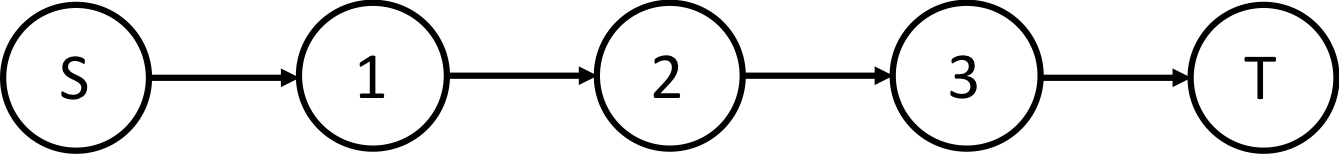
\includegraphics[width=0.8\textwidth]{serial3}
		\caption{Example of a 3-activity project}
		\label{fig:serial3}
	\end{figure}
	\noi In this example, \(I=\{1,2,3,T\}\), \(D_1=9\), \(D_2=10\), and \(D_3=7\). There is only one crashing option for each activity, so we omit the subscript to index the crashing options. We use \(e_i = 0.5\) for all \(i \in I\). The probability of the disruption not occurring is \(p^0=\frac{1}{2}\), and if a disruption occurs, it will occur at the time \(H^2 = 9.1\). The set of scenario \(\Omega = \{1\}\), where scenario 1 represents the disruption scenario. Suppose the disruption does not affect activity 1, \(d_1^1 = 0\), increases the duration of activity 2 by \(0.1\), \(d_2^1 = 0.1\), and increases the duration of activity 3 by \(6\), \(d_3^1 = 6\). We can see it is optimal to delay the start of activity 2 to \(t_2 = 9.1\). There we can observe whether the disruption happens. If the disruption occurs, it is optimal to spend the entire budget to crash activity 3, and otherwise, it is optimal to crash activity 2 with \(1\) amount of resource. The expected total project span is \(23.4\), as the optimal project span given no disruption is \(21.1\) and that under disruption is \(25.7\). If every activity starts as soon as possible, like in the deterministic problem, we cannot observe whether the disruption happens or not prior to the start of activity 2. Under this condition, the best solution is to crash activity 2 with \(1\) amount of crashing resource, and the optimal expected project span is \(24\), larger than \(23.4\). \\
	\newline
	Because it is possible for an optimal crashing plan to contain a delay for some activities, we have to set up decision variables \(t_i,\ \forall i \in I\), as the start time of each activity, rather than assume that each activity starts as soon as all of its predecessors are finished.  We summarize the reasons for such delay include:
		\begin{enumerate}
			\item Some activities might have a shorter length after the disruption. It is beneficial to wait a short period of time to capture this advantage.
			\item Even if all possible disruption magnitudes are adverse, which means they lengthen all activities, it is beneficial to delay an activity so that the crashing resource could be optimally applied according to the realization of disruption.
		\end{enumerate}
	In addition, under a stochastic disruption, it is possible that on a critical path, an activity with a smaller expected length is crashed with a larger amount of resource, while in the deterministic case, it is always optimal to start crashing from the longest one on the critical path. We present the following example to showcase this property. Suppose we have a two-activity serial network, and the disruption time follows a probability distribution shown in Figure~\ref{fig:2act}. The nominal duration of two activities is \(D_1 = 3, D_2 = 4\). The disruption does not affect the duration of activity 1, as \(d_1 = 0\), and lengthens the activity 2 by a random variable distributed in a uniform distribution with upper bound \(10\) and lower bound \(0\), as \(d_2 \sim \mathcal{U}(0,10)\). The crashing option setting is the same as the previous example, as there is only one crashing option for each activity and \(e_i = 0.5, \forall i \in I\). The total budget \(B = 1\).
		\begin{figure}[H]
			\centering
			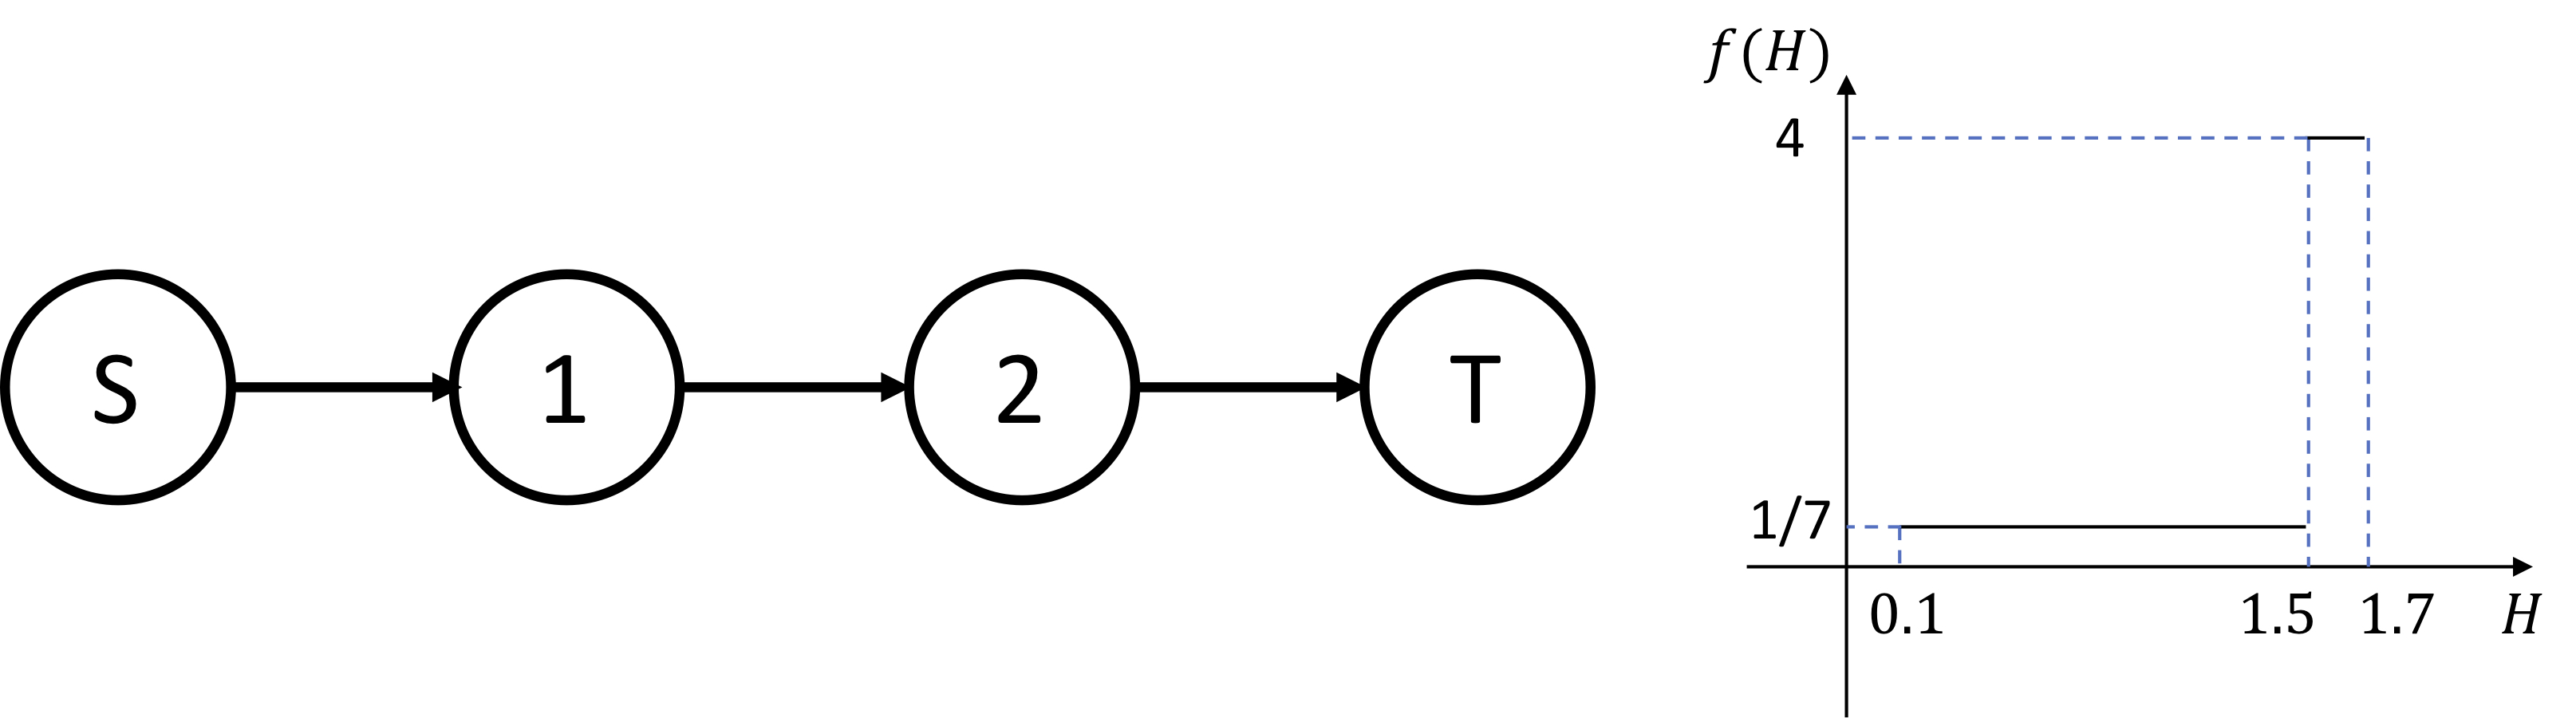
\includegraphics[width=0.8\textwidth]{2act}
			\caption{Left: an illustration of a 2-activity project; right: probability distribution function of disruption time.}
			\label{fig:2act}
		\end{figure}
	\noi In this example, the optimal solution is to crash activity 1 with one unit of resource, i.e.\,\(x_1 = 1, x_2 = 0\). Activity 1 starts at time \(t_1 = 0\) and activity 2 starts at time \(t_2 = 1.5\). The optimal expected project span is \(\mathbb{E}[t_T] = 6.5\). We can compare an alternative solution which crash activity 2 with one unit of resource, which has a longer expected duration. Crashing activity 2 matches the intuition from the deterministic case where on the critical path the activities with longer expected duration are prioritized. However, in this case with a stochastic disruption, the latter solution (\(t_1 = 0, t_2 = 3, x_1 = 0, x_2 = 1\)) yields a longer expected project span as \(\mathbb{E}[t_T] = 7.5\). The reason behind this gap is that by crashing activity 1 with one unit amount of resource, the probability of activity 2 starting before the disruption increases to \(0.8\), which prevents activity 2 from seeing the increased duration. \\
	\newline
	These examples above indicate that the crashing optimization problem with stochastic disruption has complicated nature. The intuition of deterministic crashing optimization problem does not apply here, and we need a math program model as~\eqref{prob:extensive} to solve for the best crashing plan.
	%\textcolor{blue}{NP-hardness proof.}
	%Add the conclusion of consistency. Add the proof of consistency. Prove the inconsistency of the stratified sampling method. 
	
	\section{Decomposition Method} \label{sec:decomposition}
	Model~\eqref{prob:extensive} is a two-stage stochastic mixed integer program (2SMIP). First we can decompose it into a master problem \((M)\) and a set of subproblems \((S^\omega)\), \(\omega \in \Omega\) as follows. The state variables \(t\) and \(x\) are all continuous and binary variables exist in the recourse problems, which makes recourse problems nonconvex. 
	\begin{subequations}
		\label{prob:masterOri}
		\begin{align}
		(M) \quad z^* = \min \quad &p^0 t_T + \sum_{\omega \in \Omega} p^\omega f^\omega(t,x)\\
		\text{s.t.} \quad & t_k - t_i \geq D_{i}(1 - \sum_{j \in J_i} x_{ij} e_{ij}) \qquad \qquad \forall \,i \in I, (i,k) \in \mathcal{A} \label{cons:MSep}\\
		& \sum_{i \in I} \sum_{j \in J_i} b_{ij}x_{ij} \leq B  \label{cons:MBudget}\\
		& \sum_{j \in J_i} x_{ij} \leq 1  \qquad \qquad \forall \,i \in I \label{cons:MSingleBudget}\\
		& t_i \geq 0 \qquad \qquad \forall \,i \in I\\
		& 0 \leq x_{ij} \leq 1 \qquad \qquad \forall \,i \in I, j \in J_i.
		\end{align}
	\end{subequations}
	\begin{subequations}
		\label{prob:subOri}
		\begin{align}
		(S^\omega) \qquad f^\omega(\hat{t},\hat{x}) = \min \quad & t_T \\
		& H^\omega + G_i M \geq \hat{t}_i \qquad \qquad \forall \,i \in I \label{cons:sG1}\\
		& H^\omega - (1 - G_i) M \leq \hat{t}_i \qquad \qquad \forall \,i \in I \label{cons:sG2}\\
		& t_i + G_i M_t \geq \hat{t}_i \qquad \qquad \forall \,i \in I \label{cons:stG1}\\
		& t_i - G_i M_t \leq \hat{t}_i \qquad \qquad \forall \,i \in I \label{cons:stG2}\\
		& x_{ij} + G_i \geq \hat{x}_{ij} \qquad \qquad \forall \,i \in I, j \in J_i \label{cons:sxG1}\\
		& x_{ij} - G_i \leq \hat{x}_{ij} \qquad \qquad \forall \,i \in I, j \in J_i \label{cons:sxG2}\\
		& t_k - t_i \geq D_i + d_i^\omega G_i -\sum_{j \in J_i} D_i e_{ij} x_{ij} - \sum_{j \in J_i} d_i^\omega e_{ij} z_{ij} \nonumber \\ 
		& \qquad \qquad \forall \,i \in I, j \in J_i \label{cons:subSep}\\
		& \sum_{j \in J_i} x_{ij} \leq 1 \qquad \qquad \forall \,i \in I \label{cons:subBudget1}\\
		& \sum_{i \in I}\sum_{j \in J_i} b_{ij}x_{ij} \leq B \qquad \qquad \forall \,\omega \in \Omega \label{cons:subBudget}\\
		& z_{ij} \leq G_i \qquad \qquad \forall \,i \in I, j \in J_i \label{cons:sublinearize1}\\
		& z_{ij} \leq x_{ij} \qquad \qquad \forall \,i \in I, j \in J_i \label{cons:sublinearize2}\\
		& z_{ij} \geq G_i + x_{ij} - 1 \qquad \qquad \forall \,i \in I, j \in J_i \label{cons:sublinearize3}\\
		& t_i \geq H^\omega G_i \qquad \qquad \forall\, i \in I \label{cons:subH}\\
		& 0 \leq x_{ij} \leq 1 \qquad \qquad \forall \,i \in I, j \in J_i\\
		& 0 \leq z_{ij} \leq 1 \qquad \qquad \forall \,i \in I, j \in J_i\\
		& G_i \in \{0,1\}. \qquad \qquad \forall \,i \in I. \label{cons:subInt}
		\end{align}
	\end{subequations}
	Most of the previous literature of stochastic mixed integer programming assumes a special structure or property which cannot be applied to our problem setting. For example, Gade et al. \cite{gade2014decomposition} solve 2SMIPs with pure binary first stage variables using a sequential convex approximation of recourse by a branch-and-cut process framework where Gomory cuts are added. Ahmed et al. \cite{zou2016nested} assume state variables to be binary so that the Lagrangian cuts are a tight approximation of the recourse function. Car{\o}e and Tind \cite{caroe1998shaped} solves a more general case of 2SMIP by using the MIP duality theory but the practical tractability is not verified. Qi and Sen \cite{qi2017ancestral} have mixed integer variables in both the master and the recourse problems. Parametric disjunctive cuts, derived in Chen et al. \cite{chen2012computational}, are generated to convexify recourse problems while Benders' cuts approximate recourse value functions. Although this method suits our problem settings, we implement it only to find that it does not converge in a reasonable time frame. Therefore, we need a new decomposition method that utilizes the special structure of our problem. \\
	\newline
	We can relax the integrality constraints~\eqref{cons:subInt} and solve the subproblem to obtain Benders' cuts. Although those Benders' cuts are no longer a tight approximation of the recourse function \(f^\omega(x,t), \forall \omega \in \Omega\), they still provide a valid lower bound. On the other hand, in each iteration of the Benders' decomposition, the upper bound can be obtained by solving the subproblems~\eqref{prob:subOri}, given a first stage solution. We observe that a smaller \(M\) yields a tighter gap between the upper bound and the lower bound, because we can rewrite constraints~\eqref{cons:sG1} and~\eqref{cons:sG2} as:
	\begin{equation} \label{cons:Grange}
		(\hat{t}_i - H^\omega)/M \leq G_i \leq (\hat{t}_i - H^\omega)/M + 1
	\end{equation}
	and \(G_i\) can take a wider range of value when \(M\) is larger. Therefore, sequentially tightening \(M\) is helpful to generate a tighter lower bound as the algorithm progresses. Eventually, if for a scenario we can fix the \(G_i\) for all \(i \in I\) to either 0 or 1, the Benders' cuts will be tight.\\
	\newline
	From now on we assume the scenarios \(\omega \in \Omega\) are ordered according to their time \(H^\omega\) in an ascending order. We can also observe that if we know \(\hat{t}_i \geq H^{\omega'_i}\) for some \(\omega'_i\), \(G_i\) has to take value 1 in all subproblem \(S^\omega\) where \(\omega < \omega'_i\). On the other hand if we know \(\hat{t}_i \leq H^{\omega'_i}\) for some \(\omega'_i\), \(G_i\) has to take value 0 in all subproblem \(S^\omega\) where \(\omega > \omega'_i\). These observations inform us that by bounding the value of first stage variable \(t_i,\ \forall i \in I\), we can determine the value of \(G_i\) in many subproblems, which strengthens the Benders' cuts.\\
	\newline
	We propose a decomposition algorithm to solve model~\eqref{prob:extensive}. Our method partitions the continuous feasible region of the master problem by introducing of a set of binary variables. As we refine the partition of \(t\)-space, we can generate tightened Benders' cuts to approximate the recourse function. For any crashing optimization problem, we can bound the first stage \(t_i\) variables by lower bound \(0\) and upper bound \(T_{\max} = H^{|\Omega|} + t_T^0\), where \(t_T^0\) is the longest \(S\)-\(T\) path of activity network \(\mathcal{G} = (I,\mathcal{A})\) and the arc length of \((i,j) \in \mathcal{A}\) equals to \(D_i\). This means that suppose the optimal solution of model~\eqref{prob:extensive} is denoted as \((t^*,x^*,G^{*,\cdot},t^{*,\cdot},x^{*,\cdot})\), the latter two representing the scenario specific start time and crashing decisions, we have:
	\begin{proposition} \label{prop:bounds}
		 \(t^*_i \in [0,T_{\max}],\ \forall i \in I\).
	\end{proposition}
	\begin{proof}
		Constraint~\eqref{cons:nonnegt} enforces the lower bound of this proposition. \\
		\newline 
		To derive the upper bound, 
		we first establish a feasible solution \(\tilde{t}_i = H^{|\Omega|} + t^0_i,\ \forall i \in I\), \(\tilde{x}_{ij} = 0,\ \forall i \in I, j \in J_i\) and \(\tilde{G}_i^\omega = 1,\ \forall i \in I, \omega \in \Omega\), where \(t^0_i\) represents the length of the longest \(S\)-\(i\) path of \(\mathcal{G}\). 
		If we assume that there exists some \(i \in \tilde{I}\) such that \(t_i^* > T_{\max}\), we know \(T \in \tilde{I}\). There, we can keep \(x^*\), \(G^{*,\omega}\), \(t^{*,\omega}\) and \(x^{*,\omega}\) for all \(\omega \in \Omega\) the same, and replace the \(t_i^*\) by \(\tilde{t}_i\) for all \(i \in \tilde{I}\) without violating any constraints. This yields another feasible solution which has a smaller value of \(t_T^*\) since \(T \in \tilde{I}, \tilde{t}_T = T_{\max} < t_T^*\). Therefore the new objective value obtained by this feasible solution is smaller, which contradicts the assumption that \((t^*,x^*,G^{*,\cdot},t^{*,\cdot},x^{*,\cdot})\) is an optimal solution.
	\end{proof}
	\noi Proposition~\ref{prop:bounds} indicates that all \(t_i,\ \forall i \in I\) are bounded on an interval \([0,T_{\max}]\). Since there are precedence relationships between activities, the possible range of different activities' start time can be further limited. We first set up two parameters \(H^0 = 0\) and \(H^{|\Omega| + 1} = T_{\max}\) and then define a partition of this interval for each \(i \in I\) to exploit this limitation as follows:
	\begin{definition}
		For an activity \(i \in I\), the partition of interval \([0,T_{\max}]\) is denoted by \(\mathcal{P}_i\), which is an ordered set of two-element tuples %\((\underbar{\omega}^q,\bar{\omega}^q)\), 
		\((\underbar{H}^q,\bar{H}^q)\), 
		indexed by \(q \in \mathcal{Q}_i\). We use \(\underbar{H}^q\) to specify the lower bound of \(q\)-th element of the partition and \(\bar{H}^q\) to specify its upper bound. Each of them corresponds to a disruption time of some scenario.
		%and corresponds to the lower bound scenario index and the upper bound scenario index. the disruption time of 
		The partition has the following properties:
		\begin{itemize}
			%\item \(\underbar{\omega}^1 = 0\)
			\item \(\underbar{H}^1 = H^0 = 0\)
			%\item \(\bar{\omega}^{|\mathcal{Q}_i|} = T_{\max}\)
			\item \(\bar{H}^{|\mathcal{Q}_i|} = H^{|\Omega| + 1} = T_{\max}\)
			%\item \(\bar{\omega}^q = \underbar{\omega}^{q + 1}\).
			\item \(\bar{H}^q = \underbar{H}^{q + 1}\).
		\end{itemize}
	\end{definition}
	\noi A simple example of such partition can be illustrated in Figure~\ref{fig:simplePart}. In this example we have five scenarios \(\Omega = \{1,2,3,4,5\}\), ordered by the disruption time. The partition has three elements, each illustrated by a box with dashed lines and represent a part of the interval. For partition element \(1\), the lower bound scenario index is \(0\) and the upper bound scenario index is \(2\), which means the range corresponding to it is lower bounded by \(H^0 = 0\) and upper bounded by \(H^2\).
	\begin{figure}[H]
		\centering
		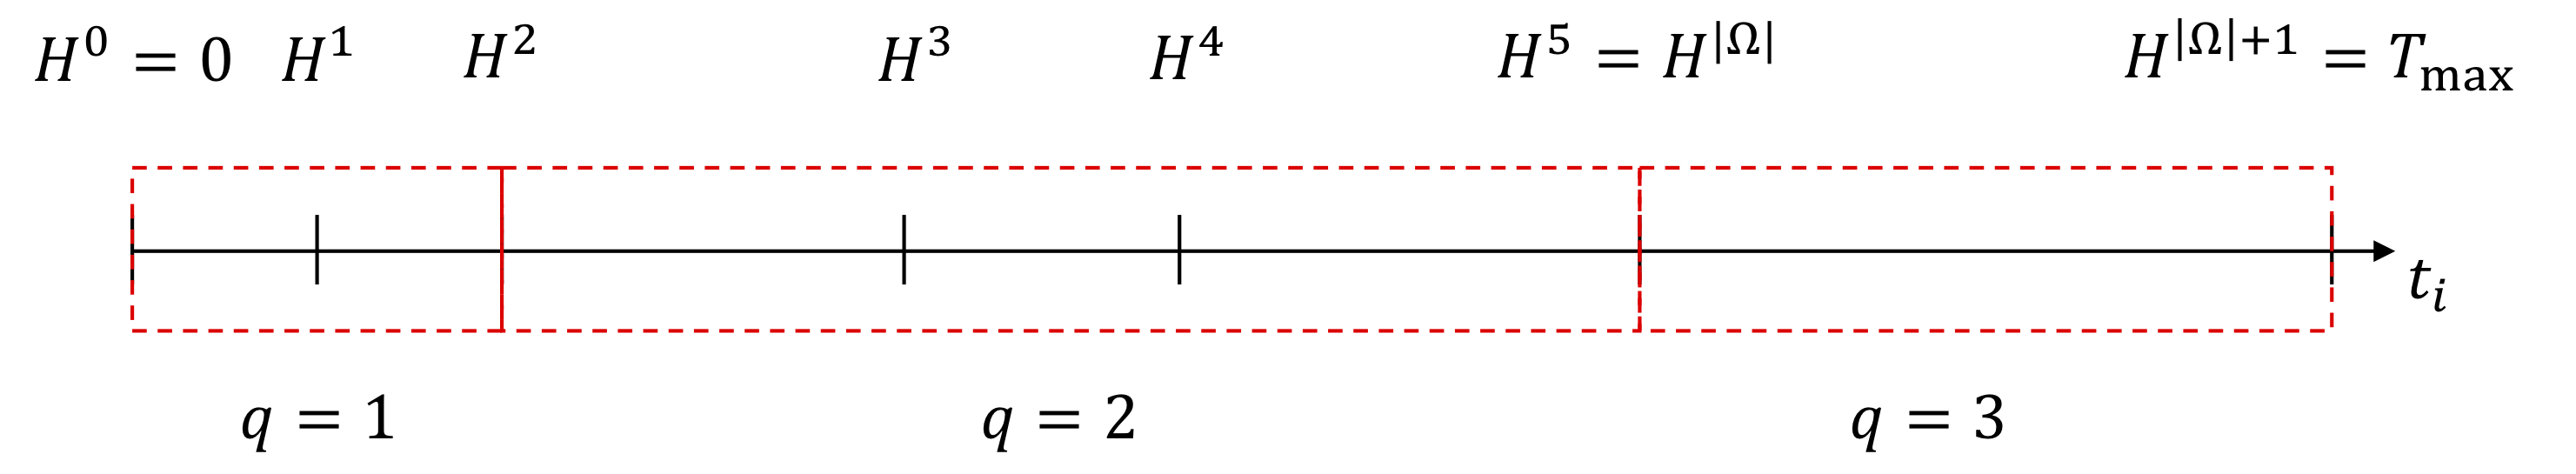
\includegraphics[width=0.8\textwidth]{simplePart}
		\caption{An illustration of partition on interval \([0,T_{\max}]\).}
		\label{fig:simplePart}
	\end{figure}
	\noi For each activity \(i \in I\), with the partition \(\mathcal{P}_i\) defined, we can see the start time \(t_i\) of the master problem lies in the range specified by one element of \(\mathcal{P}_i\). We introduce an indicator \(y_i^q\), \(\forall i \in I, q \in \mathcal{Q}_i\) in the first stage:
	\begin{equation}
		y_i^q = \begin{cases}
			%1 & \text{if \(t_i \in [H^{\underbar{\omega}^q},H^{\bar{\omega}^q}]\)}\\
			1 & \text{if \(t_i \in [\underbar{H}^q,\bar{H}^q]\)}\\
			0 & \text{otherwise}
		\end{cases}
		\qquad \forall i \in I, q \in \mathcal{Q}_i,
	\end{equation}
	and we use the following constraints to represent this relationship:
	\begin{subequations} \label{cons:yCons}
		\begin{align}
			%& \sum_{q \in \mathcal{Q}_i} H^{\underbar{\omega}^q} y_i^{q} \leq t_i \leq \sum_{q \in \mathcal{Q}_i} H^{\bar{\omega}^q} y_i^{q} \qquad \qquad \forall i \in I \label{cons:tyBounds}\\
			& \sum_{q \in \mathcal{Q}_i} \underbar{H}^q y_i^{q} \leq t_i \leq \sum_{q \in \mathcal{Q}_i} \bar{H}^q y_i^{q} \qquad \qquad \forall i \in I \label{cons:tyBounds}\\
			& \sum_{q \in \mathcal{Q}_i} y_i^q = 1 \qquad \qquad \forall i \in I. \label{cons:sumy1}
		\end{align}
	\end{subequations}
	In constraint~\eqref{cons:sumy1}, we enforce that \(t_i\) can only lie in one of the ranges specified by the partition, as only one of \(y_i^q\) can take value \(1\) for each \(i \in I\). Depending on the value of \(y_i^q\), we can write the bounds of the such range as in~\eqref{cons:tyBounds}. \\
	\newline
	The benefit of setting up the \(y\) variables is to obtain tighter bounds for \(t_i\) than the generic bounds \([0,T_{\max}]\) in Proposition~\ref{prop:bounds}. Suppose solving the master problem provides a solution \(\hat{y}_i^{\tilde{q}}, \forall i \in I, q \in \mathcal{Q}_i \). Then we can replace the big-\(M\) in constraints~\eqref{cons:sG1} and~\eqref{cons:sG2} of the scenario with moderate \(M_i^{\omega,+}\) and \(M_i^{\omega,-}\) because introducing variables \(y\) gives us better bounds on \(t_i\):
	\begin{subequations}
		\begin{align}
			%& M_i^{\omega,+} = \sum_{q \in \mathcal{Q}_i} H^{\bar{\omega}^q} \hat{y}_i^q - H^\omega\\
			%& M_i^{\omega,-} = H^\omega - \sum_{q \in \mathcal{Q}_i} H^{\underbar{\omega}^q} \hat{y}_i^q,
			& M_i^{\omega,+} = \sum_{q \in \mathcal{Q}_i} \bar{H}^q \hat{y}_i^q - H^\omega\\
			& M_i^{\omega,-} = H^\omega - \sum_{q \in \mathcal{Q}_i} \underbar{H}^q \hat{y}_i^q,
		\end{align}
	\end{subequations}
	and the constraints~\eqref{cons:sG1} and~\eqref{cons:sG2} become:
	\begin{subequations} \label{cons:newBoundsm}
		\begin{align}
			%H^\omega + G_i \left(\sum_{q \in \mathcal{Q}_i} H^{\bar{\omega}^q} \hat{y}_i^q - H^\omega \right) \geq \hat{t}_i \qquad \qquad \forall i \in I\\
			%H^\omega - (1 - G_i) \left(H^\omega - \sum_{q \in \mathcal{Q}_i} H^{\underbar{\omega}^q} \hat{y}_i^q \right) \leq \hat{t}_i \qquad \qquad \forall i \in I.
			H^\omega + G_i \left(\sum_{q \in \mathcal{Q}_i} \bar{H}^q \hat{y}_i^q - H^\omega \right) \geq \hat{t}_i \qquad \qquad \forall i \in I\\
			H^\omega - (1 - G_i) \left(H^\omega - \sum_{q \in \mathcal{Q}_i} \underbar{H}^q \hat{y}_i^q \right) \leq \hat{t}_i \qquad \qquad \forall i \in I.
		\end{align}
	\end{subequations}
	The multiplication of \(G_i \hat{y}_i^q\) makes the dual of subproblem no longer linear of \(y\). To fix this, since \(\hat{y}_i^q\) is binary and \(G_i\) for all \(i \in I, q \in \mathcal{Q}_i\), we can introduce variables \(F_i^q\) to linearize the bilinear term and rewrite constraints~\eqref{cons:newBoundsm} as follows:
	\begin{subequations} \label{cons:newBoundsmlin}
		\begin{align}
			%H^\omega + \sum_{q \in \mathcal{Q}_i} H^{\bar{\omega}^q} F_i^q - H^\omega G_i \geq \hat{t}_i \qquad \qquad \forall i \in I \label{cons:FG1}\\
			%G_i H^\omega - \sum_{q \in \mathcal{Q}_i} H^{\underbar{\omega}^q} F_i^q \leq \hat{t}_i - \sum_{q \in \mathcal{Q}_i} H^{\underbar{\omega}^q} \hat{y}_i^q \qquad \qquad \forall i \in I \label{cons:FG2}\\
			%F_i^q \leq G_i \qquad \qquad \forall i \in I, q \in \mathcal{Q}_i \label{cons:FGlin1}\\
			%F_i^q \leq \hat{y}_i^q \qquad \qquad \forall i \in I, q \in \mathcal{Q}_i \label{cons:FGlin2}\\
			%F_i^q \geq G_i + \hat{y}_i^q - 1 \qquad \qquad \forall i \in I, q \in \mathcal{Q}_i. \label{cons:FGlin3}
			H^\omega + \sum_{q \in \mathcal{Q}_i} \bar{H}^q F_i^q - H^\omega G_i \geq \hat{t}_i \qquad \qquad \forall i \in I \label{cons:FG1}\\
			G_i H^\omega - \sum_{q \in \mathcal{Q}_i} \underbar{H}^q F_i^q \leq \hat{t}_i - \sum_{q \in \mathcal{Q}_i} \underbar{H}^q \hat{y}_i^q \qquad \qquad \forall i \in I \label{cons:FG2}\\
			F_i^q \leq G_i \qquad \qquad \forall i \in I, q \in \mathcal{Q}_i \label{cons:FGlin1}\\
			F_i^q \leq \hat{y}_i^q \qquad \qquad \forall i \in I, q \in \mathcal{Q}_i \label{cons:FGlin2}\\
			F_i^q \geq G_i + \hat{y}_i^q - 1 \qquad \qquad \forall i \in I, q \in \mathcal{Q}_i. \label{cons:FGlin3}
		\end{align}
	\end{subequations}
	In the subproblem, for each activity \(i \in I\), there is only one \(\hat{q} \in \mathcal{Q}_i\) such that \(\hat{y}_i^{\hat{q}} = 1\), which means \(\hat{t}_i \in 
	%[H^{\underbar{\omega}^{\hat{q}}},H^{\bar{\omega}^{\hat{q}}}]\). 
	[\underbar{H}^{\hat{q}},\bar{H}^{\hat{q}}]\). 
	We examine the validity and effectiveness result of these tightened constraints. For validity, we check if constraints~\eqref{cons:newBoundsm} matches the logic when \(G_i\) is binary, while for effectiveness, we need to compare the feasible range of \(G\) in constraints~\eqref{cons:Grange} and that specified by constraints~\eqref{cons:newBoundsm}. \\
	\newline
	For a specific \(i \in I\), constraints~\eqref{cons:newBoundsm} can be rewritten using \(\hat{q}\):
	\begin{subequations} \label{cons:sGnew}
		\begin{align}
		%H^\omega + G_i \left( H^{\bar{\omega}^{\hat{q}}} - H^\omega \right) \geq \hat{t}_i \label{cons:sGnew1}\\
		%H^\omega - (1 - G_i) \left(H^\omega - H^{\underbar{\omega}^{\hat{q}}} \right) \leq \hat{t}_i. \label{cons:sGnew2}
		H^\omega + G_i \left( \bar{H}^{\hat{q}} - H^\omega \right) \geq \hat{t}_i \label{cons:sGnew1}\\
		H^\omega - (1 - G_i) \left(H^\omega - \underbar{H}^{\hat{q}} \right) \leq \hat{t}_i. \label{cons:sGnew2}
		\end{align}
	\end{subequations}
	For a scenario \(\omega \in \Omega\), there are three possible positions of \(H^\omega\) relative to this range with \(\hat{y}_i^{\hat{q}} = 1\): 
	%\(H^\omega \in [H^{\underbar{\omega}^{\hat{q}}},H^{\bar{\omega}^{\hat{q}}}]\), \(H^\omega < H^{\underbar{\omega}^{\hat{q}}}\), or \(H^\omega > H^{\bar{\omega}^{\hat{q}}}\). 
	\(H^\omega \in [\underbar{H}^{\hat{q}},\bar{H}^{\hat{q}}]\), \(H^\omega < \underbar{H}^{\hat{q}}\), or \(H^\omega > \bar{H}^{\hat{q}}\). 
	When \(G_i = 1\), the left-hand side of constraint~\eqref{cons:sGnew1} is \(\bar{H}^{\hat{q}}\) and the left-hand side of constraint~\eqref{cons:sGnew2} is \(H^\omega\). When \(G_i = 0\), the left-hand side of constraint~\eqref{cons:sGnew1} is \(H^\omega\), and the left-hand side of constraint~\eqref{cons:sGnew2} is 
	%\(H^{\underbar{\omega}^{\hat{q}}}\).
	\(\underbar{H}^{\hat{q}}\).
	\begin{enumerate}
		\item 
			\(H^\omega \in
			 %[H^{\underbar{\omega}^{\hat{q}}},H^{\bar{\omega}^{\hat{q}}}]\): 
			 [\underbar{H}^{\hat{q}},\bar{H}^{\hat{q}}]\): 
			 we can see that if \(\hat{t}_i \geq H^\omega\), by logic \(G_i\) should take value \(1\). Constraints~\eqref{cons:sGnew} match \(\hat{t}_i \geq H^\omega\) for \(G_i = 1\) and is violated for \(G_i = 0\). Similar validity results hold if \(\hat{t}_i < H^\omega\). In addition, the possible value \(G_i\) can take changes from the one shown in~\eqref{cons:Grange} to:
			\begin{equation}
			%\left(\hat{t}_i - H^\omega \right)/\left( H^{\bar{\omega}^{\hat{q}}} - H^\omega \right) \leq G_i \leq (\hat{t}_i - H^\omega)/\left(H^\omega - H^{\underbar{\omega}^{\hat{q}}} \right) + 1
			\left(\hat{t}_i - H^\omega \right)/\left( \bar{H}^{\hat{q}} - H^\omega \right) \leq G_i \leq (\hat{t}_i - H^\omega)/\left(H^\omega - \underbar{H}^{\hat{q}} \right) + 1 \label{cons:case1}
			\end{equation}
			Since the value of \(M\) decreases compared to constraints~\eqref{cons:Grange}, when \(\hat{t}_i \geq H^\omega\), the lower bound increases and upper bound is \(1\). When \(\hat{t}_i < H^\omega\), the upper bound decreases and the lower bound is \(0\). Therefore, the feasible range of \(G_i\) for each \(i \in I\) shrinks, which achieves the goal to tighten the subproblem relaxation.
		\item 
			%\(H^\omega < H^{\underbar{\omega}^{\hat{q}}}\): 
			\(H^\omega < \underbar{H}^{\hat{q}}\): 
			we can see \(G_i = 1\) is feasible and \(G_i = 0\) violates constraint~\eqref{cons:sGnew1}. The possible value \(G_i\) can take becomes:
			\begin{subequations}
				\begin{align}
				%G_i \geq \left(\hat{t}_i - H^\omega \right)/\left( H^{\bar{\omega}^{\hat{q}}} - H^\omega \right)\\
				%G_i \geq (\hat{t}_i - H^\omega)/\left(H^\omega - H^{\underbar{\omega}^{\hat{q}}} \right) + 1.
				G_i \geq \left(\hat{t}_i - H^\omega \right)/\left( \bar{H}^{\hat{q}} - H^\omega \right) \label{cons:case2eqn1}\\
				G_i \geq (\hat{t}_i - H^\omega)/\left(H^\omega - \underbar{H}^{\hat{q}} \right) + 1. \label{cons:case2eqn2}
				\end{align}
			\end{subequations}
			Notice that the inequality~\eqref{cons:case2eqn2} is always weaker than~\eqref{cons:case2eqn1} because the right-hand side of~\eqref{cons:case2eqn2} is smaller than 0 while the right-hand side of~\eqref{cons:case2eqn1} is positive. Similar to Case 1, the lower bound increases compared to using a large \(M\) and the upper bound is \(1\), and we achieve a tightened relaxation.
		\item 
			%\(H^\omega > H^{\bar{\omega}^{\hat{q}}}\): 
			\(H^\omega > \bar{H}^{\hat{q}}\): 
			we can see \(G_i = 0\) is feasible and \(G_i = 1\) violates constraint~\eqref{cons:sGnew2}. The possible value \(G_i\) can take becomes:
			\begin{subequations}
				\begin{align}
				%G_i \leq \left(\hat{t}_i - H^\omega \right)/\left( H^{\bar{\omega}^{\hat{q}}} - H^\omega \right)\\
				%G_i \leq (\hat{t}_i - H^\omega)/\left(H^\omega - H^{\underbar{\omega}^{\hat{q}}} \right) + 1.
				G_i \leq \left(\hat{t}_i - H^\omega \right)/\left( \bar{H}^{\hat{q}} - H^\omega \right) \label{cons:case3eqn1}\\
				G_i \leq (\hat{t}_i - H^\omega)/\left(H^\omega - \underbar{H}^{\hat{q}} \right) + 1. \label{cons:case3eqn2}
				\end{align}
			\end{subequations}
			Notice that the inequality~\eqref{cons:case3eqn1} is always weaker than~\eqref{cons:case3eqn2} because the right-hand side of~\eqref{cons:case3eqn1} is greater than 1 while the right-hand side of~\eqref{cons:case3eqn2} is between 0 and 1. Similar to Case 1, the upper bound decreases compared to using a large \(M\) and the lower bound is \(0\), and we achieve a tightened relaxation.
	\end{enumerate}
	The tightened constraints~\eqref{cons:newBoundsm} is shown to have validity and effectiveness properties. However, for the latter two situations, 
	%\(H^\omega < H^{\underbar{\omega}^{\hat{q}}}\) and \(H^\omega > H^{\bar{\omega}^{\hat{q}}}\), 
	\(H^\omega < \underbar{H}^{\hat{q}}\) and \(H^\omega > \bar{H}^{\hat{q}}\), 
	\(G_i\) can still take fractional value. We further tighten the formulation by adding two constraints involving \(y\), such that if the subproblems belonging to those two situations, \(G_i\) can be fixed as either \(0\) or \(1\). For scenario \(\omega \in \Omega\), suppose solving the master problem provides the solution \(\hat{y}_i^q, \forall i \in I, q \in \mathcal{Q}_i\), we have:
		\begin{equation}\label{cons:subyG}
			%\sum_{q \in \mathcal{Q}_i, H^\omega \leq H^{\underbar{\omega}^q}} \hat{y}_i^q \leq G_i \leq 1 - \sum_{q \in \mathcal{Q}_i, H^\omega \geq H^{\bar{\omega}^q}} \hat{y}_i^q \qquad \forall i \in I 
			\sum_{q \in \mathcal{Q}_i, H^\omega \leq \underbar{H}^q} \hat{y}_i^q \leq G_i \leq 1 - \sum_{q \in \mathcal{Q}_i, H^\omega \geq \bar{H}^q} \hat{y}_i^q \qquad \forall i \in I 
		\end{equation}
	Again we check the validity and the effectiveness result of constraints~\eqref{cons:subyG} for the three situations listed above:
	\begin{enumerate}
		\item 
			%\(H^\omega \in [H^{\underbar{\omega}^{\hat{q}}},H^{\bar{\omega}^{\hat{q}}}]\): 
			\(H^\omega \in [\underbar{H}^{\hat{q}},\bar{H}^{\hat{q}}]\): 
			the lower bound is \(0\) since \(y_i^q = 0\) for all elements of partition left of \(\hat{q}\), and the upper bound is \(1\) because \(y_i^q = 0\) for all elements of partition right of \(\hat{q}\). Therefore, \(0 \leq G_i \leq 1\) is valid.
		\item 
			%\(H^\omega < H^{\underbar{\omega}^{\hat{q}}}\): 
			\(H^\omega < \underbar{H}^{\hat{q}}\): 
			the lower bound is \(1\) since the summation term, 
			%\(\sum_{q \in \mathcal{Q}_i, H^\omega \leq H^{\underbar{\omega}^q}} \hat{y}_i^q\), includes \(y_i^{\hat{q}}\), 
			\(\sum_{q \in \mathcal{Q}_i, H^\omega \leq \underbar{H}^q} \hat{y}_i^q\), includes \(y_i^{\hat{q}}\), 
			which forces \(G_i = 1\). This matches the logic since \(\hat{t}_i \geq H^\omega\).
		\item 
			\(H^\omega > \bar{H}^{\hat{q}}\): the upper bound is \(1\) since the summation term, \(\sum_{q \in \mathcal{Q}_i, H^\omega \geq \bar{H}^q} \hat{y}_i^q\), includes \(y_i^{\hat{q}}\), which forces \(G_i = 0\). This matches the logic since \(\hat{t}_i \leq H^\omega\).
	\end{enumerate}
	With the addition of constraints~\eqref{cons:newBoundsmlin} and~\eqref{cons:subyG} in the subproblems, we present the tightened version of subproblems as follows: 
	\begin{subequations}
		\label{prob:subTightened}
		\begin{align}
		(S_{\mathcal{P}}^\omega) \qquad g^\omega_{\mathcal{P}}(\hat{t},\hat{x},\hat{y}) = \min \quad & t_T \\
		\text{s.t.} \quad & H^\omega + \sum_{q \in \mathcal{Q}_i} H^{\bar{\omega}^q} F_i^q - H^\omega G_i \geq \hat{t}_i \qquad \qquad \forall i \in I \label{cons:sFG1t}\\
		& G_i H^\omega - \sum_{q \in \mathcal{Q}_i} \underbar{H}^q F_i^q \leq \hat{t}_i - \sum_{q \in \mathcal{Q}_i} \underbar{H}^q \hat{y}_i^q \qquad \qquad \forall i \in I \label{cons:sFG2t}\\
		& F_i^q \leq G_i \qquad \qquad \forall i \in I, q \in \mathcal{Q}_i \label{cons:sFGlin1t}\\
		& F_i^q \leq \hat{y}_i^q \qquad \qquad \forall i \in I, q \in \mathcal{Q}_i \label{cons:sFGlin2t}\\
		& F_i^q \geq G_i + \hat{y}_i^q - 1 \qquad \qquad \forall i \in I, q \in \mathcal{Q}_i. \label{cons:sFGlin3t}\\
		& G_i \geq \sum_{q \in \mathcal{Q}_i, H^\omega \leq \underbar{H}^q} \hat{y}_i^q \qquad \qquad \forall i \in I \label{cons:syG1t}\\
		& G_i \leq 1 - \sum_{q \in \mathcal{Q}_i, H^\omega \geq \bar{H}^q} \hat{y}_i^q \qquad \qquad \forall i \in I \label{cons:syG2t}\\
		& \text{Constraints~\eqref{cons:stG1}-\eqref{cons:subH}}\\
		& 0 \leq x_{ij} \leq 1 \qquad \qquad \forall \,i \in I, j \in J_i\\
		& 0 \leq z_{ij} \leq 1 \qquad \qquad \forall \,i \in I, j \in J_i\\
		& 0 \leq G_i \leq 1. \qquad \qquad \forall \,i \in I. \label{cons:G01t}
		\end{align}
	\end{subequations}
	Suppose we solve the subproblems \((S_{\mathcal{P}}^\omega)\) for every \(\omega \in \Omega\) and generate a linear cut indexed by \(\ell\), where coefficients \(\pi,\lambda\) and \(\gamma\) can be calculated based on the dual variables obtained:
	\begin{equation} \label{cons:cut}
		\theta^\omega \geq v^{\omega,\ell} + \sum_{i \in I} \pi_i^{\omega,\ell} (t_i - \hat{t}_i^{\ell}) + \sum_{i \in I} \sum_{j \in J_i} \lambda_{ij}^{\omega,\ell} (x_{ij} - \hat{x}_{ij}^{\ell}) + \sum_{i \in I} \sum_{q \in \mathcal{Q}^{\ell}_i} \gamma_{i,q}^{\omega,\ell} \left( y_i^{q} - \hat{y}_i^{q,\ell} \right).
	\end{equation}
	Since the subproblem is a linear relaxation, \(\theta^\omega\) is a lower approximation of \(f^\omega\) for the current partition. However, since the validity result depends on the current partition, the cut needs to be modified once the partition is updated to retain the validity result. We assume that the update only refines the partition for each \(i \in I\):
	\begin{definition} \label{definition:refinement}
		For two partitions \(\mathcal{P}^1_i\) and \(\mathcal{P}^2_i\), indexed by \(\mathcal{Q}^1_i\) and \(\mathcal{Q}^2_i\) respectively, where \(\mathcal{P}^2_i\) is a refinement of \(\mathcal{P}^1_i\), we have:
		\begin{equation*}
		\forall q^2 \in \mathcal{Q}^2_i, \exists q^1 \in \mathcal{Q}^1_i \text{ s.t. } \bar{H}^{q^1} \geq \bar{H}^{q^2} \text{ and } \underbar{H}^{q^1} \leq \underbar{H}^{q^1}.
		\end{equation*}
	\end{definition}
	\noi Suppose at the current iteration for each \(i \in I\), the partition is \(\mathcal{P}_i\) indexed by \(\mathcal{Q}_i\), and this partition is updated from past partitions by only a sequence of refinement defined in Definition~\ref{definition:refinement}. Therefore, we can find a set of elements of the current partition,  \(\mathcal{P}_i\) refined from the \(q\)-th element in the partition \(\mathcal{P}^\ell_i\) in the previous iteration \(\ell\). We name such set as a ``descendant set", denoted by \(\Delta_i(\ell,q)\). Cut~\eqref{cons:cut} can then be updated to the following form so that the \(y\) variable has a proper dimension matching the current partition:
	\begin{align} \label{cons:updatedcut}
		& \theta^\omega \geq v^{\omega,\ell} + \sum_{i \in I} \pi_i^{\omega,\ell} (t_i - \hat{t}_i^{\ell}) + \sum_{i \in I} \sum_{j \in J_i} \lambda_{ij}^{\omega,\ell} (x_{ij} - \hat{x}_{ij}^{\ell}) + \nonumber \\
		& \qquad \sum_{i \in I} \sum_{q \in \mathcal{Q}^{\ell}_i} \gamma_{i}^{\omega,\ell,q} \left( \sum_{\tilde{q} \in \Delta_i(\ell,q)} y_i^{\tilde{q}} - \hat{y}_i^{q,\ell} \right) \qquad \forall \ell = 1,2, \dots.
	\end{align}
	We show that, given a partition, \(\mathcal{P}\), which is updated from sequential refinement, \(\mathcal{P}^\ell, \ell = 1,2,\dots\), the cut~\eqref{cons:updatedcut} is a valid lower approximation for function \(g\):
	\begin{proposition} \label{prop:validity}
		Suppose we have a partition, \(\mathcal{P}\), which is indexed by sets \(\mathcal{Q}\), and the sequence of partitions, \(\{\mathcal{P}^\ell\}_{\ell = 1}\), each of which is indexed by sets \(\mathcal{Q}^\ell\). Assuming \(\mathcal{P}\) is a refinement of \(\mathcal{P}^\ell\) for every \(\ell = 1,2, \dots\), for any \(\omega \in \Omega\), we have
		\begin{align} \label{cons:validlb}
			&g^\omega_{\mathcal{P}}(t,x,y) \geq v^{\omega,\ell} + \sum_{i \in I} \pi_i^{\omega,\ell} (t_i - \hat{t}_i^{\ell}) + \sum_{i \in I} \sum_{j \in J_i} \lambda_{ij}^{\omega,\ell} (x_{ij} - \hat{x}_{ij}^{\ell}) + \nonumber \\ 
			& \qquad \qquad \sum_{i \in I} \sum_{q \in \mathcal{Q}^{\ell}_i} \gamma_{i}^{\omega,\ell,q} \left( \sum_{\tilde{q} \in \Delta_i(\ell,q)} y_i^{\tilde{q}} - \hat{y}_i^{q,\ell} \right) \qquad \forall \ell = 1,2, \dots. 
		\end{align}
		at any given feasible \((t,x,y)\).
	\end{proposition}
	\begin{proof}
		We denote the recourse function corresponding to the partition \(\mathcal{P}^{\ell}\) as \(g^\omega_{\mathcal{P}^\ell}(t,x,y)\), where \(y\) has the correct dimension according to \(\mathcal{P}^\ell\). We first prove that 
		\begin{equation} \label{cons:gglb}
			g^\omega_{\mathcal{P}}(t,x,y) \geq g^{\omega}_{\mathcal{P}^\ell}(t,x,\tilde{y}) \qquad \forall \ell = 1,2,\dots
		\end{equation}
		where \[\tilde{y}_i^{q} =  \sum_{\tilde{q} \in \Delta_i(\ell,q)} y_i^{\tilde{q}} \qquad  \forall i \in I, q \in \mathcal{Q}^\ell_i. \]
		Suppose for an \(\omega \in \Omega\) and a \((t,x,y)\), we solve the problem \(S_{\mathcal{P}}^\omega\) and obtain the optimal solution \((t^{\omega,*},x^{\omega,*},G^{\omega,*},F^{\omega,*})\). It is easy to see that by transforming \(F^{\omega,*}\) to \(\tilde{F}^{\omega,*}\) with \[\tilde{F}^{\omega,*,q}_i = \sum_{\tilde{q} \in \Delta_i(\ell,q) }F_i^{\omega,*,\tilde{q}} \qquad  \forall i \in I, q \in \mathcal{Q}^\ell_i;\]
		thus, we obtain a feasible solution \((t^{\omega,*},x^{\omega,*},G^{\omega,*},\tilde{F}^{\omega,*})\) to the recourse problem corresponding to the partition \(\mathcal{P}^\ell\). Therefore, inequality~\eqref{cons:gglb} holds. Furthermore, the cut generated at partition \(\mathcal{P}^\ell\) is
		\[\theta^\omega \geq v^{\omega,\ell} + \sum_{i \in I} \pi_i^{\omega,\ell} (t_i - \hat{t}_i^{\ell}) + \sum_{i \in I} \sum_{j \in J_i} \lambda_{ij}^{\omega,\ell} (x_{ij} - \hat{x}_{ij}^{\ell}) + \sum_{i \in I} \sum_{q \in \mathcal{Q}^{\ell}_i} \gamma_{i}^{\omega,\ell,q} \left( y_i^{q} - \hat{y}_i^{q,\ell} \right),\]
		 which means that for any feasible \((t,x,\tilde{y})\), we have 
		 \begin{equation} \label{cons:validglb}
		 	g^\omega_{\mathcal{P}^\ell}(t,x,\tilde{y}) \geq v^{\omega,\ell} + \sum_{i \in I} \pi_i^{\omega,\ell} (t_i - \hat{t}_i^{\ell}) + \sum_{i \in I} \sum_{j \in J_i} \lambda_{ij}^{\omega,\ell} (x_{ij} - \hat{x}_{ij}^{\ell}) + \sum_{i \in I} \sum_{q \in \mathcal{Q}^{\ell}_i} \gamma_{i}^{\omega,\ell,q} \left( \tilde{y}_i^{q} - \hat{y}_i^{q,\ell} \right).
		 \end{equation}
		 By substituting \(\tilde{y}\) by \(y\) and combining inequalities~\eqref{cons:gglb} and~\eqref{cons:validglb}, we obtain the result of~\eqref{cons:validlb}.
	\end{proof}
	\noi Proposition~\ref{prop:validity} states that if we perform a proper modification on the \(y\) variables to all cuts generated in the past, the modified cuts~\eqref{cons:updatedcut} will be a valid lower approximation for the current recourse function. Therefore, we incorporate the modified cuts~\eqref{cons:updatedcut} in our master problem, given a partition \(\mathcal{P}\) indexed by \(\mathcal{Q}\), which is shown as follows:
	\begin{subequations} \label{prob:masterTightened}
		\begin{align}
		(M_{\mathcal{P}}) \quad z_{\mathcal{P}}^* = \min \quad &p^0 t_T + \sum_{\omega \in \Omega} p^\omega \theta^{\omega}\\
		\text{s.t.} \quad & t_k - t_i \geq D_{i}(1 - \sum_{j \in J_i} x_{ij} e_{ij}) \qquad \qquad \forall \,i \in I, (i,k) \in \mathcal{A} \label{cons:MpSep}\\
		& \sum_{i \in I} \sum_{j \in J_i} b_{ij}x_{ij} \leq B  \label{cons:MpBudget}\\
		& \sum_{j \in J_i} x_{ij} \leq 1  \qquad \qquad \forall \,i \in I \label{cons:MpSingleBudget}\\
		& \sum_{q \in \mathcal{Q}_i} H^{\underbar{\omega}^q} y_i^{q} \leq t_i \leq \sum_{q \in \mathcal{Q}_i} H^{\bar{\omega}^q} y_i^{q} \qquad \qquad \forall i \in I\\
		& \sum_{q \in \mathcal{Q}_i} y^q_i = 1 \qquad \qquad \forall i \in I \label{cons:MpY1}\\
		& \theta^\omega \geq v^{\omega,\ell} + \sum_{i \in I} \pi_i^{\omega,\ell} (t_i - \hat{t}_i^{\ell}) + \sum_{i \in I} \sum_{j \in J_i} \lambda_{ij}^{\omega,\ell} (x_{ij} - \hat{x}_{ij}^{\ell}) \nonumber \\
		&\qquad + \sum_{i \in I} \sum_{q \in \mathcal{Q}^{\ell}_i} \gamma_{i}^{\omega,\ell,q} \left( \sum_{\tilde{q} \in \Delta_i(\ell,q)}y_i^{\tilde{q}} - \hat{y}_i^{q,\ell} \right) \qquad  \forall \omega \in \Omega, \ell = 1, 2, \dots\\
		& y_i^q \in \{0,1\} \qquad \qquad \forall i \in I, q \in \mathcal{Q}_i\\
		& t_i \geq 0 \qquad \qquad \forall \,i \in I\\
		& 0 \leq x_{ij} \leq 1 \qquad \qquad \forall \,i \in I, j \in J_i.
		\end{align}
	\end{subequations}
	We can see that if we keep refining the partition, the generated cuts will become tighter and we will be able to provide an improving lower bound as it progresses. We refine the partition by selecting the element of \(\mathcal{P}^\ell\) indexed by \(q\), \(q \in \mathcal{Q}^\ell_i\), for each activity \(i \in I\), where for some scenarios \(\omega \in \Omega\) with \(H^\omega \in [\underbar{H}^q,\bar{H}^q]\), \(G_i^\omega\) has a fractional value, and divide the interval into three subintervals, each covering approximately the same number of scenarios. The decomposition algorithm is presented as follows:\\
	\begin{algorithm}[H]
		\caption{Decomposition algorithm to solve problem~\eqref{prob:extensive}}
		\label{alg:Cut}
		\begin{algorithmic}[1]
			\State Initialize with cut iteration number \(\ell = 0\), lower bound \(LB = 0\), upper bound \(UB = +\infty\), initial partition \(\mathcal{P}^\ell\) with its indexed set \(\mathcal{Q}^\ell\), and specified tolerance \(\epsilon > 0\) and \(\delta > 0\);
			\While{\(\frac{UB - LB}{UB} > \epsilon\)} 
			\State Solve master problem \((M_{\mathcal{P}})\) and obtain solution \(\hat{t}^{\ell}, \hat{x}^{\ell}, \hat{y}^{\ell}, \hat{\theta}^{\ell}\) and optimal value \(z_{P}^*\);
			\If{\(z_{P}^* > LB\)}
			\State Update \(LB = z_{P}^*\);
			\EndIf
			\State For each \(\omega \in \Omega\), solve problem \((S^\omega)\) and obtain \(f^{\omega}(\hat{t},\hat{x})\). 
			\State Calculate \(z^* = p^0 \hat{t}^\ell_T + \sum_{\omega \in \Omega} p^\omega f^{\omega}(\hat{t}^\ell,\hat{x}^\ell)\)
			\If{\(z^* < UB\)} 
			\State Update \(UB := z^*\) and record the best incumbent solution as \(t^* = \hat{t}^\ell, x^* = \hat{x}^\ell\) and \(y^* = \hat{y}^\ell\);
			\EndIf
			\State For each \(\omega \in \Omega\), solve problem \((S_{\mathcal{P}}^\omega)\) given \(\hat{t}^{\ell}, \hat{x}^{\ell}, \hat{y}^{\ell}, \hat{\theta}^{\ell}\) and obtain optimal value \(v^{\omega,\ell}\) and coefficients \(\pi^{\omega,\ell}, \lambda^{\omega,\ell}, \gamma^{\omega,\ell}\);
			\If{\(z^*_P < p^0 \hat{t}_T + \sum_{\omega \in \Omega} p^\omega v^{\omega,\ell} - \delta\)}
			\State Add the cuts of form~\eqref{cons:cut} to the master problem;
			\State Keep \(\mathcal{P}^{\ell + 1} = \mathcal{P}^\ell\) and \(\mathcal{Q}^{\ell + 1} = \mathcal{Q}^\ell\); 
			\State Update \(\ell = \ell + 1\);
			\Else
			\State Refine the partition and obtain the new partition \(\mathcal{P}^{\ell + 1}\) and its indexed sets \(\mathcal{Q}^{\ell + 1}\);
			\State Update \(\ell = \ell + 1\);
			\State Update the previously generated cuts in the master problem to the form of~\eqref{cons:updatedcut};
			\EndIf
			\vspace{0.1cm}
			\EndWhile{\textbf{end while}}
			\State Output \(UB\) as the optimal value of model~\eqref{prob:extensive}, and \(t^*, x^*,y^*\) as the optimal solution.
		\end{algorithmic}
	\end{algorithm}
	\noi Finally we prove Algorithm~\ref{alg:Cut} converges in finite number of iterations. Since every partition update is a refinement and we have a finite set of scenario \(\Omega\), we can prove the finite convergence of Algorithm~\ref{alg:Cut} as long as with the finest partition we reach the optimum of problem~\eqref{prob:extensive}.
	\begin{proposition} \label{prop:finestPar}
		If a partition \(\hat{\mathcal{P}}\) has indexed sets \(\hat{\mathcal{Q}}\) and for each \(i \in I\), \(|\hat{\mathcal{Q}}_i| = |\Omega|\) and \(\bar{\omega}^q = \underbar{\omega}^q + 1,\ \forall q \in \hat{\mathcal{Q}}_i\), we have \[z^* = \min_{(t,x,y) \in \mathbb{X}}\ t_T + \sum_{\omega \in \Omega} g^\omega_{\hat{\mathcal{P}}}(t,x,y),\]
		where 
		\begin{equation*}
			\mathbb{X} = \left\{(t,x,y) \left| 
			\begin{aligned}
			& \text{Constraints } \eqref{cons:MpSep}-\eqref{cons:MpY1}\\ 
			&y_i^q \in \{0,1\} \qquad \forall i \in I, q \in \hat{\mathcal{Q}}_i\\
			& t_i \geq 0 \qquad \forall i \in I\\
			& 0 \leq x_{ij} \leq 1 \qquad \forall i \in I, j \in J_i
			\end{aligned}
			\right. \right\}.
		\end{equation*}
	\end{proposition}
	\begin{proof}
		First we can consider the subproblem \((S_\mathcal{P}^\omega)\) as a partial linear relaxation of the original extensive formulation. So \(z^* \leq z^*_\mathcal{P}\) is automatically true.\\
		\newline
		Next we prove that, given the partition in Proposition~\ref{prop:finestPar}, we can construct a feasible solution, \((t^*,x^*,G^*)\), to the extensive formulation~\eqref{prob:extensive} with the same objective value from the optimal solution, \((\hat{t},\hat{x},\hat{y})\), to the problem
		\[\min_{(t,x,y) \in \mathbb{X}}\ t_T + \sum_{\omega \in \Omega} g^\omega_{\hat{\mathcal{P}}}(t,x,y).\]
		Suppose for \(i \in I\), we denote the index of partition where \(y\) variable takes value \(1\) as \(q_i\). Since \(\bar{H}^q = \underbar{H}^{q + 1},\ \forall q \in \hat{\mathcal{Q}}_i\), either \(q_i \in \{q \in \hat{\mathcal{Q}}_i \mid H^\omega \leq \underbar{H}^q\}\) or \(q_i \in \{q \in \hat{\mathcal{Q}}_i \mid H^\omega \geq \bar{H}^q\}\) is true. Thus, constraints~\eqref{cons:syG1t} and~\eqref{cons:syG2t} enforce that \(G_i\) in the problem \((S_{\hat{\mathcal{P}}}^\omega)\) takes binary value because the right-hand side expressions of those two constraints must be \(0\) or \(1\) simultaneously. This means that although subproblems are linear programs, the integrality is implied. Therefore, when we obtain the optimal solution \(\hat{G}^\omega\) from solving problems \((S_{\hat{\mathcal{P}}}^\omega)\) for each \(\omega \in \Omega\), solution \((\hat{t},\hat{x},\hat{G})\) will be feasible for the extensive formulation because \((\hat{t},\hat{x},\hat{y}) \in \mathbb{X}\) and \(G\) variables satisfy the constraints~\eqref{cons:stG1}-\eqref{cons:subH} and binary constraints. This result is equivalent to \(z_{\hat{\mathcal{P}}}^* \geq z^*\). Combining the results above we conclude that \(z^* = \min_{(t,x,y) \in \mathbb{X}}\ t_T + \sum_{\omega \in \Omega} g^\omega_{\hat{\mathcal{P}}}(t,x,y).\)
	\end{proof}
	\begin{theorem} \label{thm:converge}
		Algorithm~\ref{alg:Cut} terminates in finite number of iteration for any \(\epsilon \geq 0\). 
	\end{theorem}
	\begin{proof}
		From Proposition~\ref{prop:finestPar} we know that with the finest partition \(\hat{\mathcal{P}}\) where for each \(i \in I\), \(|\hat{\mathcal{Q}}_i| = |\Omega|\) and \(\bar{H}^q = \underbar{H}^{q + 1},\ \forall q \in \hat{\mathcal{Q}}_i\), solving the problem \(\min_{(t,x,y) \in \mathbb{X}}\ t_T + \sum_{\omega \in \Omega} g^\omega_{\hat{\mathcal{P}}}(t,x,y)\) is equivalent to solving the extensive formulation. Since there are only finite number of scenarios, it takes finite number of steps of refinement to reach the finest partition. \\
		\newline
		For each subproblem, there is only a finite number of possible values of dual variables because each corresponds to one of the finitely many different bases. This means that, for any partition \(\mathcal{P}\), the recourse function \(g^\omega_{\mathcal{P}}\) can be represented by finitely many linear cuts. Therefore, in algorithm~\ref{alg:Cut}, only a finite number of cuts are added for a finite number of partitions before \(UB = z^*\) and \(LB = z^*_{\hat{\mathcal{P}}}\) is achieved, a.k.a. \(\frac{UB - LB}{UB} = 0\).
	\end{proof}
	\begin{comment}
	\textcolor{blue}{ The materials above are the most important idea I want to convey in this section. Here are some additional results we have discussed but I haven't compiled to \LaTeX \ yet. Time allowing, I can add some stuff in maybe tonight or this coming week.
		\begin{itemize}
			\item Concavity of \(\mathbb{E}_d \left[ f(x,H,d) | H \right]\) in \(d\).
			\item The analytical form of the recourse function when all \(d\) are \([0,1]\)-uniformly distributed, all \(D\) are equal, and the crashing option can only be integer.
			\item The recourse function is a decreasing function in terms of remaining budget, given the same remaining task set.
			\item Not optimal to delay the start of activity \(i\) unless there is no investment before \(i\), given a fixed \(H\).
			\item Only optimal to delay to a possible disruption time.
		\end{itemize}
	}
	\subsection{Parallel Networks}
		\begin{itemize}
			\item Not optimal to delay when \(d_i \geq 0\) if each branch only contains a single activity.
			\item If each branch is a serial path, it is possibly beneficial to delay the start of some activities.
		\end{itemize}
	\subsection{Y Networks}
\section{Properties of the Sample Average Approximation Problem} \label{sec:consistency}
	\subsection{Cheat?}
	\subsection{Consistency and Convergence Results}
	\subsection{IID vs. Stratified Sampling}

	\subsection{Deterministic Counterparts}
		List the test results of INFORMS presentation. State the fact that the fully stochastic makes great improvement over its deterministic counterparts.
		
%\section{Stochastic Mixed Integer Program Extension}
\end{comment}

\section{Experimental Results} \label{sec:results}
%	\textcolor{blue}{Test results:
%	\begin{itemize}
%		\item Describe the test examples: where do they come from, number of nodes, how are they generated.
%		\item Cite Sen's paper and describe the implementation.
%		\item Results.
%	\end{itemize}}
	In this section, we address the following questions with our computational results:
	\begin{enumerate}
		\item What is the value of model~\eqref{prob:extensive} that takes account of randomness in both timing and magnitude of a disruption? In other words, what are other alternative solutions that are easier to obtain but possibly inferior? How does the quality of the solution to model~\eqref{prob:extensive} compare to those alternative solutions?
		\item How does the solution quality improve as the number of samples used in sample average approximation increases? 
		\item What is the time improvement of Algorithm~\ref{alg:Cut} compared to solving extensive formulation~\eqref{prob:extensive} using state-of-the-art MIP solvers? Other algorithms solving 2SMIP with mixed binary recourse?
	\end{enumerate}
	We first introduce the PERT network used for test and distribution information used to characterize uncertainty in Section~\ref{subsec:example}. In Section~\ref{subsec:value} we construct a series of deterministic and semi-deterministic alternatives to model~\eqref{prob:extensive}, perform out-of-sample tests, and present the better quality result of the solution to model~\eqref{prob:extensive} compared to the alternative ones. We test the effect of different simulation budgets on solution quality and computational performance in Section~\ref{subsec:budget}. Finally in Section~\ref{subsec:time} we present the computational advantage of Algorithm~\ref{alg:Cut} compared to solving extensive formulation.\\
	\newline
	All tests are run on a server with 20 Intel Xeon cores at 3.1 GHz and 256 GB of RAM. All models are constructed using version 0.18.0 of the JuMP package \cite{DunningHuchetteLubin2017} on the Julia platform. All linear programs and mixed integer programs are solved by Gurobi 8.01 \cite{gurobi2016} with default parameters.
	
	\subsection{Test Cases Construction} \label{subsec:example}
	%	\textcolor{blue}{Where we find our tests:
	%		\begin{itemize}
	%			\item Plambeck paper: Case 11
	%			\item V42: Case 14
	%			\item Case 19 from Elmgrabhy
	%			\item Case 55 from Elmgrabhy
	%			\item Randomized network 75, 100 nodes
	%			\item Plambeck paper: Case 110
	%	\end{itemize}}
	\noi Although it is easy to construct an activity network with randomly distributed disruption time and magnitude, not all instances constructed can well illustrate properties of our problem. Therefore, we construct our test cases based on the activity networks used in the previous literature, which have been shown of research value. We use an activity network from Plambeck et al.~\cite{plambeck1996sample} with 11 activities, % and the other with 110 activities. 
	one from Elmgrabhy \cite{Elmaghraby77} with 19 activities, and 
	 %and the other with 55 activities. 
	 we also manually create one activity network with 14 activities. 
	 %and generate two random networks with 75 and 100 activities, respectively using \textcolor{blue}{RanGen toolbox}. 
	 In the following section, we use ``Case \(X\)" to denote the test case with \(X\) activities.\\
	\newline
	For every test case, the timing of disruption follows a lognormal distribution since its value has to be nonnegative. The disruption magnitude of activities follows an exponential distribution of which the parameter differs among activities. The exponential distribution can best model the drastic change caused by a disruption.
	\subsection{Value of a Fully Stochastic Model} \label{subsec:value}
	In this section, we compare the quality of five solutions obtained under different possible problem settings to show the value of modeling random timing and magnitude of the disruption. First, we can solve a deterministic project crashing problem assuming no disruption occurs (denoted as ``DET"). Three semi-stochastic alternatives can be constructed assuming: both timing and magnitude of the disruption are deterministic at their expected values (denoted as ``EXP"), the timing is random but the magnitude is at its expected value (denoted as ``\(H\)Only"), and the magnitude is random but the timing is at its expected value (denoted as ``\(d\)Only"). Finally, we construct the full stochastic model where both the timing and the magnitude are random (denoted as ``FULL"). To generate those five solutions, we use a sample of size \(500\). We can obtain a point estimation for the upper bound by plugging each of these solutions in the SAA problem with the original \(500\) samples, and we call this estimation as ``in-sample" since these samples are also used to obtain solutions. We also sample 20 batches of samples of \(|\Omega| = 5000\), and obtain another upper bound estimation, and its confidence interval, by plugging each of those solutions in every batch of the sample. We present the comparison of different solutions of Case 11 in Figure~\ref{fig:value}.
	\begin{figure}[H]
		\centering
		\includegraphics[width=0.8\textwidth]{case11_altValues}
		\caption{Comparison of quality of alternative solutions to the problem~\eqref{prob:extensive}}
		\label{fig:value}
	\end{figure}
	Figure~\ref{fig:value} shows that the solution quality is poor without considering the uncertainty of disruption timing. When we assume the disruption timing is uncertain, the computational effort required to obtain ``\(H\)Only" solution and the fully stochastic solution is on the same level, since we need to include the same number of binary variables. To further test whether having a fully stochastic model is the best, we run a pair-wise \(t\)-test. The null hypothesis is that whether the difference between the upper bound generated by one alternative solution and that generated by the fully stochastic solution is less than 0. The result of the \(t\)-test is displayed in Table~\ref{table:value}.
	\begin{table}[H]
		\centering
		\begin{tabular}{c c c c c c}
			\hline
			& Det & Exp & dOnly & HOnly & Full\\
			In-sample obj & 118.35 & 112.33 & 114.91 & 98.82 & 98.82 \\
			Out-of-sample obj mean & 114.44 & 108.04 & 110.346 & 98.75 & 98.75 \\
			t-test result (p-value) & \(< 10^{-5}\) & \(< 10^{-5}\)& \(< 10^{-5}\)&  \(0.001945\)& -\\
			\hline
		\end{tabular}
		\caption{Compare optimal values from alternatives of the disruption model}
		\label{table:value}
	\end{table}
	The pair-wise \(t\)-test rejects all null hypotheses, which shows that the difference between an alternative solution is significantly larger than the fully stochastic solution. We can conclude the fully stochastic solution is the best solution, and this justifies the value of having a fully stochastic model, albeit its complexity.
	\subsection{Simulation Budget} \label{subsec:budget}
	We first examine the quality of solutions generated from different sizes of samples. It is well known that the objective value obtained by SAA approaches the objective function of the original problem as the sample size grows to infinity, and the expected value of the SAA objective value improves as the sample size increases~\cite{shapiro2009lectures}. However, when the sample size increases, the computational cost increases as well. Understanding how the solution quality changes according to different sample sizes is important to help us decide a proper sample size while achieving a decent solution. For each test case in Section~\ref{subsec:example}, we first obtain \(20\) batches of the optimal solution to model~\ref{prob:extensive} by Algorithm~\ref{alg:Cut}, with sample sizes \(|\Omega| \in \{10, 50, 75, 100, 200, 300, 400, 500\}\). For each of those solutions, we test against a set of \(5000\) samples and obtain the object value as a point estimation of the upper bound for each batch. We can also obtain the \(95\%\) confidence interval of the lower bound and the upper bound estimation for each sample size. We present the result for Case 19 in Figure~\ref{fig:budget}.
	\begin{figure}[H]
		\centering
		\includegraphics[width=0.8\textwidth]{case19_budget_ublb}
		\caption{Confidence intervals of the lower/upper bound estimation for sample size \(|\Omega| \in \{10, 50, 75, 100, 200, 300, 400, 500\}\)}
		\label{fig:budget}
	\end{figure}
	We can see the gap between the upper bound and the lower bound estimation is decreasing as the sample size increases. A decent solution can be obtained by sampling a moderate number of samples, since the upper bound estimation stabilizes when the sample size is greater than \(100\). However, to achieve a good lower bound estimation requires a large number of samples. This comes from the nature of our uncertainty model, as we need to consider both timing and magnitude of the disruption. 
	\subsection{Computational Performance} \label{subsec:time}
	In this section we present the computational result of our decomposition method. 
	%We solve each of the test cases with different sizes of samples \(|\Omega| \in \{100,200,300,400,500,1000\}\) (\(20\) times for each sample size) and show the mean computational time. 
	We can see the benefit of our decomposition method in Figure~\ref{fig:time}, with the example of Case 11. In each master iteration, we solve a master problem with a small number of binary variables. Although we need to solve multiple rounds of the master problem and the number of binary variables is increasing since the partition is refined in every iteration, we still can observe a significant improvement by using our proposed decomposition method, especially when the sample size is large.
	\begin{figure}[H]
		\centering
		\includegraphics[width=0.8\textwidth]{case11_time}
		\caption{Computational performance for sample size \(|\Omega| \in \{100, 200, 300, 400, 500,1000\}\)}
		\label{fig:time}
	\end{figure}
\section{Conclusions} \label{sec:conclusions}
	In this paper, we establish the concept of stochastic disruption and formulate a two-stage stochastic mixed integer program to model a project crashing optimization problem under the influence of single disruption. We use examples to illustrate the counterintuitive properties of our problem that it is possible to delay the start or crash a shorter activity to accelerate the whole project. Moreover, the computational results justify the need to use a two-stage stochastic mixed integer program to model this problem. It is computationally challenging to solve a two-stage stochastic mixed integer program with binary variables in the second stage. Therefore, we propose a decomposition method which uses the logic relationship to generate strong linear programming relaxation of recourse problems and sequentially partitions the master feasible regions to generate Benders' cuts. The proposed method can significantly improve the computational performance, especially for the large sample sizes, which we show is often required to obtain a good solution/estimation of bounds.\\
	\newline
	There are multiple possible extensions of the results in this paper. First, there is still room to improve the computational performance of the decomposition method. Currently, the refining process is to divide the partition element with fractional \(G\) values into three partitions evenly. This can be enhanced by learning the right partition points so that the lower bound can be tightened faster. In addition, we are working on exploiting the network structures to improve the quality of cuts or prune partitions. 
\bibliographystyle{plainnat}
\bibliography{PERT_Bib}

\end{document}